%%%%%%%%%%%%%%%%%%%%%%%%%%%%%%%%%%%%%%%%%
% MEIA Dissertation
% LaTeX Template
% (Jan/2022)
%
% Adapted once again to MEIA/ISEP style (Jan(2022) by:
%  Luiz Faria (lef@isep.ipp.pt)
%
% Adapted to TMDEI/ISEP style (Dec/2015) by
%  Nuno Pereira (nap@isep.ipp.pt) and
%  Paulo Baltarejo (pbs@isep.ipp.pt)
%
% Based on MastersDoctoralThesis Version 1.2 by Vel (vel@latextemplates.com) and
% Johannes Böttcher, downloaded from (21/11/15):
% http://www.LaTeXTemplates.com
%
% This template is originally based on a template by:
% Steve Gunn (http://users.ecs.soton.ac.uk/srg/softwaretools/document/templates/)
% Sunil Patel (http://www.sunilpatel.co.uk/thesis-template/)
%
% Template license:
% CC BY-NC-SA 3.0 (http://creativecommons.org/licenses/by-nc-sa/3.0/)
%
%%%%%%%%%%%%%%%%%%%%%%%%%%%%%%%%%%%%%%%%%
%
%----------------------------------------------------------------------------------------
%	PACKAGES AND OTHER DOCUMENT CONFIGURATIONS
%----------------------------------------------------------------------------------------

\documentclass[
11pt, % The default document font size, options: 10pt, 11pt, 12pt
%oneside, % Avoid blank pages inserted to force chapters onto right-hand pages (enable twoside later if you need duplex printing)
english, % english for English;
%portuguese,% for Portuguese; delete temporary files if you change language (e.g. 'make clean; make')
singlespacing, % Single line spacing, alternatives: onehalfspacing or doublespacing (for drafting/reading purposes)
%draft, % Uncomment to enable draft mode (no pictures, no links, overfull hboxes indicated)
%nolistspacing, % If the document is onehalfspacing or doublespacing, uncomment this to set spacing in lists to single
liststotoc, % Uncomment to add the list of figures/tables/etc to the table of contents (not recommended)
%toctotoc, % Uncomment to add the main table of contents to the table of contents (not recommended)
parskip, % Add space between paragraphs (recommended)
%nohyperref, % Uncomment to not load the hyperref package (not recommended)
nohyperreflinkcolor, % hyperref links are not colored (comment to color links, for example to produce an electronic-only version)
headsepline, % Uncomment to get a line under the header
]{meia-style} % The class file specifying the document structure

\usepackage{tikz} % Required for creating graphics programmatically (can be removed if not used)
%\usetikzlibrary{arrows} % Required for fancy arrows in TiKZ graphics (can be removed if not used)

\usepackage{pgfplots} % Required for drawing high--quality function plots (can be removed if not used)
\pgfplotsset{compat=newest}

%
% Next you have examples of admissable citation styles; we recomend using the authoryear-comp citation style (which resembles Harvard); don't forget to only uncomment one
%

% Line breaking: lets TeX stretch inter-word space slightly instead of letting long words/citations poke into the margin
\setlength{\emergencystretch}{3em}

% authoryear-comp: recommended citation style (e.g. (Buendía, 1860), (Buendía 1910, Arcadio 1940))
\usepackage[style=authoryear-comp,backend=biber]{biblatex} % BibLaTeX with Biber backend (recommended); citations are author-year, bibliography alphabetical

% numeric citation style (e.g. [1], [1-3])
%\usepackage[style=numeric-comp,sorting=none,backend=bibtex]{biblatex} % BibLaTeX with BibTeX backend (numeric citations, bibliography ordered by appearance)

% alphabetic citation style (e.g. [Buendía10], [Buendía10, Arcadio40])
%\usepackage[style=alphabetic,sorting=none,backend=bibtex]{biblatex} % BibLaTeX with BibTeX backend (alphabetic citations, bibliography ordered by appearance)

\usepackage{makecell}

\addbibresource{mainbibliography.bib} % The filename of the bibliography

%\makeglossaries % build the glossary
\makenoidxglossaries % build the glossary (to work with overleaf)
% All acronyms and glossary terms should be written in this file.
% Keep definitions beginner-friendly (assume a reader outside NLP/AI/education research).

% -----------------------------------------------------------------------------
% Acronyms
% -----------------------------------------------------------------------------

\newacronym{AI}{AI}{Artificial Intelligence}
\newacronym{NLP}{NLP}{Natural Language Processing}
\newacronym{AWE}{AWE}{Automated Writing Evaluation}
\newacronym{AES}{AES}{Automated Essay Scoring}
\newacronym{GEC}{GEC}{Grammatical Error Correction}
\newacronym{ITS}{ITS}{Intelligent Tutoring System}
\newacronym{EDM}{EDM}{Educational Data Mining}

\newacronym{LLM}{LLM}{Large Language Model}




\newacronym{LSTM}{LSTM}{Long Short-Term Memory}
\newacronym{BiLSTM}{BiLSTM}{Bidirectional Long Short-Term Memory}
\newacronym{CNN}{CNN}{Convolutional Neural Network}
\newacronym{CRF}{CRF}{Conditional Random Field}

\newacronym{BERT}{BERT}{Bidirectional Encoder Representations from Transformers}

\newacronym{CoNLL}{CoNLL}{Conference on Natural Language Learning}
\newacronym{BEA}{BEA}{Workshop on Innovative Use of NLP for Building Educational Applications}
\newacronym{MTwo}{M2}{MaxMatch (M2) scorer}
\newacronym{ERRANT}{ERRANT}{Error Annotation Toolkit}

\newacronym{K12}{K--12}{Kindergarten to Grade 12 education}
\newacronym{NER}{NER}{Named Entity Recognition}
\newacronym{NUCLE}{NUCLE}{National University of Singapore Corpus of Learner English}

% -----------------------------------------------------------------------------
% Glossary terms (non-acronyms)
% -----------------------------------------------------------------------------

\newglossaryentry{nucleCorpus}{
	name={NUCLE corpus},
	description={A corpus of English learner essays created at the National University of Singapore; it is widely used as a benchmark dataset for grammatical error correction (e.g., in the CoNLL-2014 shared task)}}

\newglossaryentry{learnerCorpus}{
	name={learner corpus},
	description={A collection of texts or responses produced by learners (e.g., language learners or students), often annotated to study typical errors and development patterns}}

\newglossaryentry{errorDetection}{
	name={error detection},
	description={The task of identifying where errors occur in a text (and sometimes what type they are), without necessarily producing a corrected version}}

\newglossaryentry{errorCorrection}{
	name={error correction},
	description={The task of producing a corrected text from an input text that contains errors, often framed as a generation problem in NLP}}

\newglossaryentry{sequenceLabeling}{
	name={sequence labeling},
	description={A modeling setup where each token in a sequence (e.g., each word) receives a label, such as an error tag or a part-of-speech tag}}

\newglossaryentry{token}{
	name={token},
	description={A basic unit used by NLP models, such as a word, subword piece, punctuation mark, or character, depending on the tokenizer}}

\newglossaryentry{span}{
	name={span},
	description={A contiguous segment of text, such as a phrase or a range of tokens, often used when labeling multi-token errors}}

\newglossaryentry{pretraining}{
	name={pretraining},
	description={Training a model on a large generic dataset to learn general language patterns before adapting it to a specific task}}

\newglossaryentry{finetuning}{
	name={fine-tuning},
	description={Continuing training of a pretrained model on task-specific data to adapt it to a target task and domain}}

\newglossaryentry{domainAdaptation}{
	name={domain adaptation},
	description={Techniques to make a model trained on one domain (e.g., general web text) work better on another (e.g., student writing) }}

\newglossaryentry{syntheticData}{
	name={synthetic data},
	description={Artificially generated training data (e.g., by injecting errors or corruptions) used to augment scarce real labeled data}}

\newglossaryentry{misconception}{
	name={misconception},
	description={A systematic misunderstanding that leads to consistent incorrect reasoning patterns, rather than an occasional slip or typo}}

\newglossaryentry{formativeAssessment}{
	name={formative assessment},
	description={Assessment used to support learning during the learning process, typically through timely feedback and guidance rather than final grading}}

\newglossaryentry{modelTracing}{
	name={model tracing},
	description={An ITS approach that compares a student’s step-by-step actions to a cognitive model of how problems can be solved, enabling immediate difficulty identification and feedback}}

\newglossaryentry{precision}{
	name={precision},
	description={Among the items predicted as positive (e.g., predicted errors), the fraction that are actually correct}}

\newglossaryentry{recall}{
	name={recall},
	description={Among the items that are actually positive (e.g., real errors), the fraction that a system successfully finds}}

\newglossaryentry{fscore}{
	name={F-score},
	description={A family of metrics that combine precision and recall; common choices include \(F_1\) (equal weight) and \(F_{0.5}\) (higher weight on precision)}}
 % the command makenoidxglossaries requires that the glossary entries must be defined in the preamble

%----------------------------------------------------------------------------------------
%	THESIS INFORMATION
%----------------------------------------------------------------------------------------

\thesistitle{System for Error Detection and Learning Difficulties} % Your thesis title, this is used in the title, print it elsewhere with \ttitle

\thesissubtitle{Automatic Analysis of Student Responses in Primary and Secondary Education} % Your thesis subtitle, this is used in the title, print it elsewhere with \tsubtitle

\author{Miguel Mendes Rodrigues} % Your name, this is used in the title page, print it elsewhere with \authorname

\studentnumber{1181734}

%\subjectarea{Área de Especialização} % Specialisation area, used in the title page, print it elsewhere with \areaname

\supervisor{Doctor Luís Filipe de Oliveira Gomes, Assistant Researcher, Polytechnic of Porto - School of Engineering} % Your supervisor's name, this is used in the title page, print it elsewhere with \supname


\committeepresident{Doctor Luiz Felipe Rocha de Faria, Associate Professor, Polytechnic of Porto - School of Engineering} % Name of the president of the evaluation committee, print it elsewhere with \presidentname

\committeemembers{Doctor António Constantino Lopes Martins, Associate Professor, Polytechnic of Porto - School of Engineering\\Doctor Luís Filipe de Oliveira Gomes, Assistant Researcher, Polytechnic of Porto - School of Engineering} % Name of the evaluation committee members (up to four), print it elsewhere with \committee

\keywords{Natural Language Processing, Educational Data Mining, Error Analysis, Symbolic Artificial Intelligence, Student Profiling, Synthetic Data Generation}

\university{\href{http://www.isep.ipp.pt}{Instituto Superior de Engenharia do Porto}} % Your university's name and URL, this is used in the title page and abstract, print it elsewhere with \univname

\department{Departamento de Engenharia Inform\'atica} % Your department's name and URL, this is used in the title page and abstract, print it elsewhere with \deptname

\thesisdate{Porto, September 2026}

\hypersetup{pdftitle=\ttitle} % Set the PDF's title to your title
\hypersetup{pdfauthor=\authorname} % Set the PDF's author to your name
\hypersetup{pdfkeywords=\keywordnames} % Set the PDF's keywords to your keywords

\begin{document}

%----------------------------------------------------------------------------------------
%	FRONT MATTER
%----------------------------------------------------------------------------------------

% Include the frontmatter of your thesis here
% we include the glossary here (frontmatter is included with \input, so this command is as if it was in main.tex)
%% All acronyms and glossary terms should be written in this file.
% Keep definitions beginner-friendly (assume a reader outside NLP/AI/education research).

% -----------------------------------------------------------------------------
% Acronyms
% -----------------------------------------------------------------------------

\newacronym{AI}{AI}{Artificial Intelligence}
\newacronym{NLP}{NLP}{Natural Language Processing}
\newacronym{AWE}{AWE}{Automated Writing Evaluation}
\newacronym{AES}{AES}{Automated Essay Scoring}
\newacronym{GEC}{GEC}{Grammatical Error Correction}
\newacronym{ITS}{ITS}{Intelligent Tutoring System}
\newacronym{EDM}{EDM}{Educational Data Mining}

\newacronym{LLM}{LLM}{Large Language Model}




\newacronym{LSTM}{LSTM}{Long Short-Term Memory}
\newacronym{BiLSTM}{BiLSTM}{Bidirectional Long Short-Term Memory}
\newacronym{CNN}{CNN}{Convolutional Neural Network}
\newacronym{CRF}{CRF}{Conditional Random Field}

\newacronym{BERT}{BERT}{Bidirectional Encoder Representations from Transformers}

\newacronym{CoNLL}{CoNLL}{Conference on Natural Language Learning}
\newacronym{BEA}{BEA}{Workshop on Innovative Use of NLP for Building Educational Applications}
\newacronym{MTwo}{M2}{MaxMatch (M2) scorer}
\newacronym{ERRANT}{ERRANT}{Error Annotation Toolkit}

\newacronym{K12}{K--12}{Kindergarten to Grade 12 education}
\newacronym{NER}{NER}{Named Entity Recognition}
\newacronym{NUCLE}{NUCLE}{National University of Singapore Corpus of Learner English}

% -----------------------------------------------------------------------------
% Glossary terms (non-acronyms)
% -----------------------------------------------------------------------------

\newglossaryentry{nucleCorpus}{
	name={NUCLE corpus},
	description={A corpus of English learner essays created at the National University of Singapore; it is widely used as a benchmark dataset for grammatical error correction (e.g., in the CoNLL-2014 shared task)}}

\newglossaryentry{learnerCorpus}{
	name={learner corpus},
	description={A collection of texts or responses produced by learners (e.g., language learners or students), often annotated to study typical errors and development patterns}}

\newglossaryentry{errorDetection}{
	name={error detection},
	description={The task of identifying where errors occur in a text (and sometimes what type they are), without necessarily producing a corrected version}}

\newglossaryentry{errorCorrection}{
	name={error correction},
	description={The task of producing a corrected text from an input text that contains errors, often framed as a generation problem in NLP}}

\newglossaryentry{sequenceLabeling}{
	name={sequence labeling},
	description={A modeling setup where each token in a sequence (e.g., each word) receives a label, such as an error tag or a part-of-speech tag}}

\newglossaryentry{token}{
	name={token},
	description={A basic unit used by NLP models, such as a word, subword piece, punctuation mark, or character, depending on the tokenizer}}

\newglossaryentry{span}{
	name={span},
	description={A contiguous segment of text, such as a phrase or a range of tokens, often used when labeling multi-token errors}}

\newglossaryentry{pretraining}{
	name={pretraining},
	description={Training a model on a large generic dataset to learn general language patterns before adapting it to a specific task}}

\newglossaryentry{finetuning}{
	name={fine-tuning},
	description={Continuing training of a pretrained model on task-specific data to adapt it to a target task and domain}}

\newglossaryentry{domainAdaptation}{
	name={domain adaptation},
	description={Techniques to make a model trained on one domain (e.g., general web text) work better on another (e.g., student writing) }}

\newglossaryentry{syntheticData}{
	name={synthetic data},
	description={Artificially generated training data (e.g., by injecting errors or corruptions) used to augment scarce real labeled data}}

\newglossaryentry{misconception}{
	name={misconception},
	description={A systematic misunderstanding that leads to consistent incorrect reasoning patterns, rather than an occasional slip or typo}}

\newglossaryentry{formativeAssessment}{
	name={formative assessment},
	description={Assessment used to support learning during the learning process, typically through timely feedback and guidance rather than final grading}}

\newglossaryentry{modelTracing}{
	name={model tracing},
	description={An ITS approach that compares a student’s step-by-step actions to a cognitive model of how problems can be solved, enabling immediate difficulty identification and feedback}}

\newglossaryentry{precision}{
	name={precision},
	description={Among the items predicted as positive (e.g., predicted errors), the fraction that are actually correct}}

\newglossaryentry{recall}{
	name={recall},
	description={Among the items that are actually positive (e.g., real errors), the fraction that a system successfully finds}}

\newglossaryentry{fscore}{
	name={F-score},
	description={A family of metrics that combine precision and recall; common choices include \(F_1\) (equal weight) and \(F_{0.5}\) (higher weight on precision)}}
 % the command makenoidxglossaries requires that the glossary entries must be defined in the preamble (to be compatible with overleaf)

\frontmatter % Use roman page numbering style (i, ii, iii, iv...) for the pre-content pages

\pagestyle{plain} % Default to the plain heading style until the thesis style is called for the body content

%----------------------------------------------------------------------------------------
%	TITLE PAGE
%----------------------------------------------------------------------------------------

\maketitlepage

%----------------------------------------------------------------------------------------
%	STATEMENT OF INTEGRITY
%----------------------------------------------------------------------------------------

\begin{soi}

% here you put the statement of integrity in the main language of the work. Choose one option.
\vspace{1cm}

% if the main language is English:

I hereby declare that I have conducted this academic work with integrity.

I have not plagiarised or applied any form of undue use of information or falsification of results along the process leading to its elaboration.

Therefore, the work presented in this document is original and was authored by me, having not been previously used for any other purpose.

I further declare that I have fully acknowledged the Code of Ethical Conduct of P.PORTO.

ISEP, Porto, September 2026

\vspace{2cm}

\begin{flushright}
\rule{7cm}{0.4pt}\\
\authorname{} (\studnumber)
\end{flushright}


\end{soi}


%----------------------------------------------------------------------------------------
%	DEDICATION  (optional)
%----------------------------------------------------------------------------------------
%
%\dedicatory{For/Dedicated to/To my\ldots}
% \begin{dedicatory}
% [Dedicatory to be added by the author]
% \end{dedicatory}

%----------------------------------------------------------------------------------------
%	ABSTRACT PAGE
%----------------------------------------------------------------------------------------

\begin{abstract}

This thesis addresses the automatic detection of error patterns linked to learning difficulties in typed student responses, under the practical constraint that annotated data for the target population is scarce. It proposes a modular, text-only architecture with three components: a Transformer-based sequence-labeling module for difficulty-linked linguistic errors (phonological, orthographic, segmentation), a hybrid symbolic and machine-learning module for arithmetic procedural bugs, and an unsupervised profiling module that aggregates detections into interpretable difficulty profiles, understood as statistical profiles over observable error patterns.

Data scarcity is addressed with rule-based synthetic error generation staged in a synthetic-to-real training curriculum. Evaluation on real learner text yields a span-level F-score (the harmonic mean of precision and recall) of 0.642 under a strict exact-span metric. The synthetic-data hypothesis is not supported: a multi-seed paired comparison against real-only training from scratch shows that synthetic pre-training with $10^6$ examples lowers the real-data F-score by 2.5--7 points and is at best neutral with $10^4$ examples, and a scale ablation shows that increasing synthetic volume improves in-domain performance while degrading real-data transfer. These results are consistent with the match between synthetic and authentic error distributions, not data volume, being the limiting factor.

On real writing by children with literacy difficulties, performance drops by roughly 20 F-score points, quantifying the domain gap that defines the main direction for future work; under this shift, free-text detection preserves student rankings by error volume but not by error type, which motivates a two-regime design that routes designed worksheet items to deterministic scoring and free text to the neural model.

For mathematics, on generated malrule data, exact symbolic simulation and a feature-based classifier are complementary, trading precision on modeled bugs against robustness to input noise, and the identifiability of a misconception is shown to depend on the structure of the problem posed. Difficulty profiles are supported by three analyses: recoverability in simulation, archetype-like structure in the writing of 19 real struggling children, and split-half stability of behavioral profiles on 1{,}519 real students.

A pilot-ready prototype demonstrates the pipeline end to end, including a European Portuguese instantiation of the screening mode. Throughout, the system is framed as providing non-clinical, formative information for educators, with claims sized to the evidence.

\end{abstract}

\begin{abstractotherlanguage}
% here you put the abstract in the "other language": English, if the work is written in Portuguese; Portuguese, if the work is written in English.

Esta tese aborda a deteção automática de padrões de erro associados a dificuldades de aprendizagem em respostas digitadas por alunos, sob a restrição prática de que os dados anotados para a população-alvo são escassos. Propõe-se uma arquitetura modular, baseada exclusivamente em texto, com três componentes: um módulo de etiquetagem sequencial baseado em Transformers para erros linguísticos associados a dificuldades (fonológicos, ortográficos, de segmentação), um módulo híbrido simbólico e de aprendizagem automática para erros procedimentais em aritmética, e um módulo de perfis que agrega as deteções em perfis de dificuldade interpretáveis, entendidos como perfis estatísticos sobre padrões de erro observáveis.

A escassez de dados é abordada com geração sintética de erros baseada em regras, organizada num currículo de treino sintético-para-real. A avaliação em texto real de aprendentes atinge uma medida F (média harmónica da precisão e da cobertura) de 0.642 ao nível do segmento sob uma métrica estrita. A hipótese dos dados sintéticos não é suportada: uma comparação emparelhada multi-semente com treino apenas em dados reais mostra que o pré-treino sintético com $10^6$ exemplos reduz a medida F em dados reais em 2.5--7 pontos e é, na melhor das hipóteses, neutro com $10^4$ exemplos, e uma ablação de escala mostra que aumentar o volume sintético melhora o desempenho no domínio sintético mas degrada a transferência para dados reais. Estes resultados são consistentes com a correspondência entre as distribuições de erro sintéticas e autênticas, e não o volume de dados, ser o fator limitante.

Em escrita real de crianças com dificuldades de literacia, o desempenho cai cerca de 20 pontos de medida F, quantificando o fosso de domínio que define a principal direção de trabalho futuro; sob este desvio, a deteção em texto livre preserva a ordenação dos alunos por volume de erros mas não por tipo de erro, o que motiva um desenho de dois regimes que encaminha itens de fichas de trabalho para pontuação determinística e texto livre para o modelo neuronal.

Na matemática, em dados gerados com regras de erro modeladas, a simulação simbólica exata e um classificador baseado em características são complementares, trocando precisão em erros modelados por robustez ao ruído, e mostra-se que a identificabilidade de uma conceção errónea depende da estrutura do problema apresentado. Os perfis de dificuldade são apoiados por três análises: recuperabilidade em simulação, estrutura de arquétipos na escrita de 19 crianças reais com dificuldades, e estabilidade por divisão em duas metades de perfis comportamentais em 1{,}519 alunos reais.

Um protótipo pronto para piloto demonstra a cadeia completa, incluindo uma instanciação em Português Europeu do modo de rastreio. A informação fornecida aos educadores é não-clínica e formativa, com afirmações dimensionadas à evidência.

\end{abstractotherlanguage}

%----------------------------------------------------------------------------------------
%	ACKNOWLEDGEMENTS (optional)
%----------------------------------------------------------------------------------------

% \begin{acknowledgements}

% [Acknowledgements to be added by the author]

% \end{acknowledgements}

%----------------------------------------------------------------------------------------
%	LIST OF CONTENTS/FIGURES/TABLES PAGES
%----------------------------------------------------------------------------------------

\tableofcontents % Prints the main table of contents

\listoffigures % Prints the list of figures

\listoftables % Prints the list of tables

\iflanguage{portuguese}{
\renewcommand{\listalgorithmname}{Lista de Algor\'itmos}
}
% Commented out - no algorithm environments in current thesis chapters
%\listofalgorithms % Prints the list of algorithms
%\addchaptertocentry{\listalgorithmname}


\renewcommand{\lstlistlistingname}{List of Source Code}
\iflanguage{portuguese}{
\renewcommand{\lstlistlistingname}{Lista de C\'odigo}
}
% Commented out - no lstlisting environments in current thesis chapters
%\lstlistoflistings % Prints the list of listings (programming language source code)
%\addchaptertocentry{\lstlistlistingname}



%----------------------------------------------------------------------------------------
%	ABBREVIATIONS
%----------------------------------------------------------------------------------------
%\begin{abbreviations}{ll} % Include a list of abbreviations (a table of two columns)
%%\textbf{LAH} & \textbf{L}ist \textbf{A}bbreviations \textbf{H}ere\\
%%\textbf{WSF} & \textbf{W}hat (it) \textbf{S}tands \textbf{F}or\\
%\end{abbreviations}

%----------------------------------------------------------------------------------------
%	SYMBOLS
%----------------------------------------------------------------------------------------

\begin{symbols}{ll} % Include a list of Symbols (a two column table)

$P$ & precision \\
$R$ & recall \\
$F_1$ & \(F\)-score with \(\beta=1\) (precision and recall weighted equally) \\
$F_{0.5}$ & \(F\)-score with \(\beta=0.5\) (precision weighted higher than recall) \\
$TP$ & true positives \\
$FP$ & false positives \\
$FN$ & false negatives \\
$x$ & input text (e.g., a student response) \\
$y$ & output labels (e.g., error tags per token) \\
$p_{\theta}(y\mid x)$ & model probability of \(y\) given \(x\) \\
$\mathcal{L}$ & training loss function \\

\addlinespace % Gap to separate the Roman symbols from the Greek

$\beta$ & \(F\)-score weighting parameter \\
$\theta$ & model parameters \\

\end{symbols}



%----------------------------------------------------------------------------------------
%	ACRONYMS
%----------------------------------------------------------------------------------------

\newcommand{\listacronymname}{List of Acronyms}
\iflanguage{portuguese}{
\renewcommand{\listacronymname}{Lista de Acr\'onimos}
}

%Use GLS
\glsresetall
\glsaddallunused

%\printglossary[title=\listacronymname,type=\acronymtype,style=long]
\printnoidxglossary[title=\listacronymname,type=\acronymtype,style=long] % command compatible with overleaf

\newcommand{\listglossaryname}{Glossary}
\iflanguage{portuguese}{
\renewcommand{\listglossaryname}{Gloss\'ario}
}
\printnoidxglossary[title=\listglossaryname,style=long]

%----------------------------------------------------------------------------------------
%	DONE
%----------------------------------------------------------------------------------------

\mainmatter % Begin numeric (1,2,3...) page numbering
\pagestyle{thesis} % Return the page headers back to the "thesis" style


%----------------------------------------------------------------------------------------
%	MAIN BODY
%----------------------------------------------------------------------------------------

% Include the chapters of the thesis as separate folder for each chapter
% Uncomment the lines as you write the chapters

% Chapter 1
% 
\chapter{Introduction} % Main chapter title
\label{chap:introduction} % For referencing the chapter elsewhere, use Chapter~\ref{chap:introduction}

The problem addressed by this thesis and the reasoning behind it are introduced in this chapter. Section~\ref{sec:context_motivation} describes the context and motivation, Section~\ref{sec:hypothesis} states the research hypotheses, and Section~\ref{sec:questions} lists the research questions. The general and specific objectives follow in Section~\ref{sec:objectives}, and Section~\ref{sec:structure} closes the chapter with an overview of how the rest of the document is organized.

%-------------------------------------------------------------------------------
%---------
%
\section{Context and Motivation} 
\label{sec:context_motivation}

Identifying specific errors and learning difficulties in student work is a time-consuming and challenging task for educators across primary and secondary education (K--12). Teachers must routinely interpret short answers, essays, worksheets, and problem-solving traces while balancing instruction, planning, and administrative work. Large-scale workload evidence shows why timely identification is difficult in practice: in the OECD Teaching and Learning International Survey (TALIS) 2018, lower-secondary teachers report spending a substantial working week on non-teaching tasks, including several hours per week on marking and correcting student work \parencite{OECDTALIS2018VolI}. The 2024 round of the survey extends this evidence on the demands of teaching and also reports whether and how teachers use artificial intelligence \parencite{OECDTALIS2024}. In parallel, class size in lower secondary education commonly exceeds 20 students and is considerably larger in some education systems, which increases the volume and heterogeneity of student responses that need assessment \parencite{OECDEAG2019}. When assessment occurs manually at scale, feedback tends to focus on surface correctness and completion; recurring error mechanisms that indicate persistent difficulties receive less attention. As a consequence, patterns that inform targeted support often become visible only after repeated failures or summative assessments, despite long-standing evidence that earlier identification and support prevent compounding learning gaps \parencite{SnowBurnsGriffin1998}.

A non-trivial fraction of learners experience persistent difficulties in foundational skills. Dyslexia (a specific reading disability), for example, is far from rare. A common definition, based on a reading-achievement cutoff of 1.5 standard deviations below the mean for age, identifies about 7\% of the population as dyslexic, and estimates vary with the diagnostic criteria adopted \parencite{PetersonPennington2012}. At the system level, international learning indicators point to the urgency of scalable analytical support. The World Bank has reported high rates of ``learning poverty'' (the inability to read and understand a simple text by age 10) in low- and middle-income contexts, which shows how widespread foundational difficulties become when early support is constrained \parencite{WorldBank2022LearningPoverty}. These figures motivate tools that help educators detect patterns earlier and more consistently, without replacing professional judgment or producing clinical diagnoses.

Artificial Intelligence (AI) and, more specifically, Natural Language Processing (NLP) and learning analytics offer a concrete path to scale formative assessment. In writing tasks, this goal has driven Automated Writing Evaluation (AWE) systems and error detection research that combine scoring with feedback-oriented language analysis \parencite{Bryant2023GECsurvey}. Research on error detection and Grammatical Error Correction (GEC) has benefited from shared tasks and benchmarks that enabled comparable evaluation \parencite{Ng2014,Bryant2019}. Yet these resources and the strongest-performing models are unevenly distributed across languages and educational domains, which complicates generalizable deployment in diverse educational settings \parencite{Joshi2020}. For Portuguese, recent work includes an LLM-assisted characterization of errors in a European Portuguese learner corpus \parencite{Akef2026} and a synthetic dataset for grammar correction in Brazilian Portuguese \parencite{Cabral2026}. In educational workflows, correcting a single response is rarely enough; teachers need summaries that connect error types to likely sources of difficulty and that support monitoring progress over time \parencite{RomeroVentura2024}. Large Language Models (LLMs) can generate controlled synthetic data for rare error categories and help scale development, but the educational use case demands explicit constraints on reliability and transparency, especially when the output informs instruction, not grading \parencite{Brown2020}. Recent work on the use of LLMs in education reviews both the opportunities they open for learning and teaching and the challenges that accompany them \parencite{Kasneci2023}.

In mathematics and other structured-response tasks, formative assessment goals commonly go beyond correctness to identifying systematic misconceptions and recurring procedural ``bugs'' that guide targeted remediation \parencite{VanLehn1990}. The opportunities for scalable text-based analysis are especially relevant in digital learning environments, where students submit typed responses (short answers, explanations, essays, and numeric solutions) through learning management systems, online assessments, and digital worksheets. This thesis focuses exclusively on such digital, text-only workflows. Authentic classroom assessments often include handwritten responses, but integrating handwriting recognition (OCR/HTR) introduces distinct technical challenges that are outside the scope of this work and are reserved for future research. By isolating the text analysis component, this thesis aims to establish a baseline for error detection in digital environments.\par

The main gap addressed in this thesis is the lack of teacher-oriented systems that (i) detect and classify error patterns specifically linked to learning difficulties (e.g., phonological, orthographic, and segmentation errors in language; procedural bugs and conceptual misconceptions in mathematics), (ii) aggregate these errors over time into interpretable difficulty profiles, and (iii) do so under realistic data-scarcity constraints using synthetic data augmentation. The intended outcome is actionable, non-clinical information that supports educators' formative assessment and planning without providing clinical diagnoses of learning disabilities.

\section{Research Hypothesis}
\label{sec:hypothesis}

Based on these challenges, the following hypotheses are proposed. Throughout this thesis, performance is assessed using standard evaluation measures from educational data mining (EDM) and NLP (precision, recall, \(F_1\)-score), complemented by clustering validity indicators. Inter-rater agreement measures such as Cohen's \(\kappa\) \parencite{Cohen1960} would apply to a teacher-annotation study, and qualitative educator review to a classroom pilot; neither was conducted within this thesis, and both are specified as future work (Chapter~\ref{chap:Chapter6}). The hypotheses are intentionally formulated at a high level so that model choices, integration strategies, and evaluation protocols evolve as empirical evidence and design constraints emerge during the thesis.

\begin{itemize}
    \item \textbf{Main Hypothesis (H1):} Text-based NLP models and symbolic methods, trained on a combination of authentic and synthetic student responses, can identify pedagogically meaningful error types (phonological, orthographic, and segmentation errors in language; procedural bugs and conceptual misconceptions in mathematics) with performance consistent with expert teacher annotations and established instructional taxonomies, without providing clinical diagnosis. Performance is evaluated on typed inputs using standard classification metrics (precision, recall, \(F_1\)-score).\footnote{No new teacher-annotation study was conducted; the evidence in Chapter~\ref{chap:Chapter5} measures performance against the expert-produced gold annotations of existing corpora, which tests the detection component of H1 but not its consistency with independently collected teacher judgments.}
    \item \textbf{Secondary Hypothesis (H2):} Using rule-based generators and Large Language Models (LLMs) to produce synthetic learner-error data improves the robustness and generalization of error detection and classification models in data-scarce educational scenarios. The hypothesis thus seeks to validate, for current students and in the present educational context, the benefits reported for synthetic training data in the literature (Section~\ref{sec:sota_synth}). Improvements are assessed empirically using held-out evaluation and generalization checks (e.g., cross-validation and transfer across tasks or difficulty levels).\footnote{As documented in Section~\ref{sec:method_data_llm}, LLM-based generation was considered and deliberately not adopted; the empirical evidence in Chapter~\ref{chap:Chapter5} therefore addresses the rule-based part of this hypothesis and leaves the LLM part untested.}
    \item \textbf{Secondary Hypothesis (H3):} Unsupervised pattern discovery methods aggregate recurring errors over time into meaningful student difficulty profiles that are interpretable and actionable for educators. Here too, the aim is to validate, for current students and in the present educational context, the profiling approaches reported in the EDM literature (Section~\ref{sec:sota_ethics}). Profile quality is assessed through a combination of clustering validity indices and pedagogical interpretability.\footnote{Interpretability is assessed by inspection of cluster centroids against the taxonomy (Section~\ref{sec:method_models_profile}); validation of pedagogical meaningfulness and actionability with educators was not conducted and is part of the pilot proposed in Chapter~\ref{chap:Chapter6}.}
\end{itemize}

\section{Research Questions}
\label{sec:questions}

To test the proposed hypotheses and guide the development of the system, this research seeks to answer the following questions:

\begin{enumerate}
    \item[\textbf{Q1}] Linguistic error taxonomies: What linguistic error types (phonological, orthographic, and segmentation) are observable and recurrent in the available typed learner corpora, how do their distributions differ across learner populations, and how are they best structured into a formal taxonomy suitable for automated text analysis?
    \item[\textbf{Q2}] Detection and classification models: To what extent do NLP sequence-labeling models automatically detect and classify difficulty-linked linguistic errors in typed text, as measured by span-level \(F_1\)-score against expert-produced gold annotations, including on text from the target population?
    \item[\textbf{Q3}] Mathematical misconception detection: How well do symbolic methods and simple ML classifiers identify characteristic arithmetic procedural bugs (e.g., smaller-from-larger subtraction) and fraction misconceptions (e.g., whole-number bias) from typed numeric answers?
    \item[\textbf{Q4}] Data scarcity and synthesis: In the context of limited annotated educational datasets, what combination of real student data, rule-based synthetic error generation, and LLM-based augmentation provides the most effective training set, as measured by \(F_1\)-score stability and generalization, while maintaining fidelity to authentic learner error distributions?
    \item[\textbf{Q5}] Difficulty profiling: Do aggregated error patterns cluster into stable and interpretable student difficulty profiles, and how might these profiles be presented to educators in a non-clinical format?
\end{enumerate}

\section{Objectives}
\label{sec:objectives}

Concrete goals follow from the hypotheses and questions above. A general objective states the overall aim of the work, and six specific objectives (O1--O6) split it into the tasks addressed in the following chapters, covering the error taxonomies, the data strategy, model development, and evaluation.

\subsection{General Objective}
The primary objective of this thesis is to design and evaluate an NLP-based system capable of analyzing typed student responses in primary and secondary education (K--12) to detect specific error patterns linked to learning difficulties and to infer interpretable difficulty profiles. The system should provide educators with actionable, non-clinical information to support formative assessment and pedagogical planning.

\subsection{Specific Objectives}
\begin{enumerate}
    \item[\textbf{O1}] Define and formalize error taxonomies. Identify and categorize linguistic errors (phonological, orthographic, and segmentation) and mathematical errors (procedural bugs in arithmetic, fraction misconceptions) into formal taxonomies suitable for automated detection.
    \item[\textbf{O2}] Develop a data strategy combining real and synthetic data. Design rule-based generators to produce synthetic student responses with controlled error patterns, complementing limited real educational data (LLM-based generation was considered and not adopted; Section~\ref{sec:method_data_llm}).
    \item[\textbf{O3}] Develop linguistic error detection models. Implement and evaluate NLP sequence-labeling models (e.g., fine-tuned Transformer encoders) for token-level or span-level error tagging on typed text.
    \item[\textbf{O4}] Develop mathematical misconception detection. Implement symbolic computation and template-matching methods to identify procedural bugs and conceptual misconceptions from typed numeric answers.
    \item[\textbf{O5}] Implement student difficulty profiling. Aggregate error statistics per student and apply clustering algorithms to discover interpretable difficulty profiles.
    \item[\textbf{O6}] Evaluate system performance and pedagogical utility. Define metrics (precision, recall, \(F_1\), clustering indices) for quantitative evaluation and assess interpretability for teacher-facing use by inspection of the resulting profiles (educator validation is deferred to a school pilot).
\end{enumerate}

\section{Thesis Structure}
\label{sec:structure}

The remainder of this dissertation is organized as follows. Chapter~\ref{chap:Chapter2} presents the state of the art in NLP for education, grammatical error correction and detection, mathematical error analysis, synthetic data generation for educational AI, and the pedagogical and ethical dimensions of learning-difficulty identification. This chapter positions the thesis with respect to the main gaps: (i) the underrepresentation of certain languages and local educational contexts; (ii) the limited use of synthetic data for difficulty-linked error patterns; and (iii) the tendency to focus on isolated responses, with longitudinal difficulty patterns receiving less attention.

Chapter~3 turns to the proposed error taxonomies and the data strategy. It formalizes linguistic error categories (phonological, orthographic, segmentation) and mathematical error categories (procedural bugs, fraction misconceptions). The data approach combines limited real student data with rule-based synthetic error generation (LLM-based generation was considered and deliberately not adopted), and it includes quality control procedures.

Chapter~4 covers the system architecture and its implementation: the NLP-based linguistic error detection module, the symbolic/template-based mathematical misconception detection module, and the profiling module that aggregates errors into student difficulty profiles. Implementation details are documented there.

Chapter~5 contains the experimental evaluation. Quantitative results cover error detection (precision, recall, \(F_1\), with paired bootstrap confidence intervals and multi-seed replication), domain shift to the target population, the impact and scaling behavior of synthetic data (including a real-only baseline trained without any synthetic stage), mathematical misconception detection under clean and perturbed conditions, and difficulty-profile validity (clustering recoverability and split-half stability via the Adjusted Rand Index).

Chapter~6 concludes the thesis by summarizing contributions, discussing limitations, and outlining future work, including extension to additional languages and real classroom deployment. The bibliography and appendices follow.
% Chapter 2

\chapter{State of the Art} % Main chapter title
\label{chap:Chapter2} % For referencing the chapter elsewhere, use \ref{chap:Chapter2}

%----------------------------------------------------------------------------------------

This chapter reviews research on the automatic analysis of student responses, with emphasis on (i) Natural Language Processing (NLP) for educational assessment, (ii) error detection and correction in student writing, (iii) mathematical error analysis and misconception modeling, and (iv) synthetic data strategies for data-scarce educational settings. It places the thesis within established evaluation practices and modeling paradigms, points out gaps in current work, and states what the thesis contributes \parencite{Bryant2023GECsurvey,Woolf2010,RomeroVentura2024}.

\section{NLP for education and automated assessment}
\label{sec:sota_nlp_edu}

To place the thesis within established practice, this section looks at how Natural Language Processing (NLP) has been applied to educational assessment. The account is historical first. It then moves to the benchmarks and shared tasks used to compare systems, the architectures used for assessment and diagnosis, and the language coverage and deployment gaps that remain beyond English.

\subsection{Historical evolution of NLP in education}
\label{sec:sota_nlp_edu_history}

Automated assessment has passed through several distinct technical paradigms (Figure~\ref{fig:nlp_evolution}).

\begin{figure}[ht]
\centering
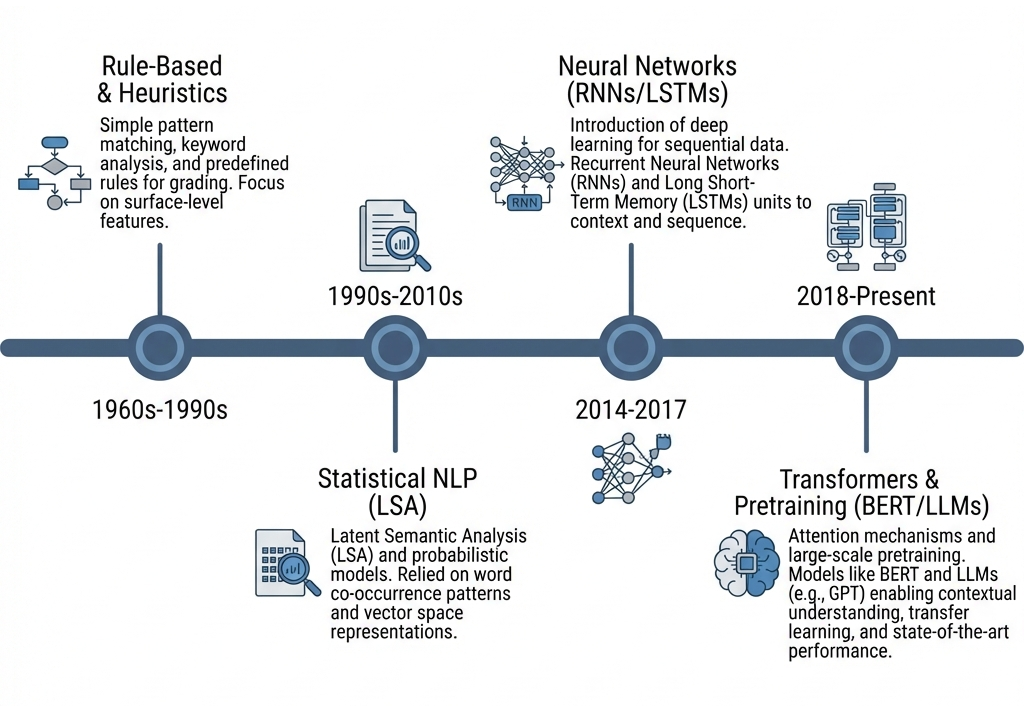
\includegraphics[width=1.0\textwidth]{figures/nlp_evolution_timeline.png}
\caption{Timeline showing the evolution of automated assessment from rule-based heuristics to modern Transformer-based architectures.}
\label{fig:nlp_evolution}
\end{figure}

Educational NLP initially focused on rule-based spell checking and grammar checking embedded in writing tools. These systems provided scalable surface-level feedback but offered limited diagnostic insight into why learners struggle. With the rise of Automated Essay Scoring (AES) and Automated Writing Evaluation (AWE), models increasingly learned to predict holistic or rubric-aligned scores from linguistic features extracted from corpora of human-scored responses. This motivated datasets for grading open-ended student writing such as the FCE corpus \parencite{YannakoudakisBriscoeMedlock2011,Bryant2023GECsurvey}.

Neural sequence models then enabled finer-grained signals, such as token-level error detection posed as a sequence labeling problem \parencite{ReiYannakoudakis2016}. In parallel, transformer architectures and large-scale pretraining shifted many educational NLP pipelines toward contextual representations that transfer across tasks. This shift improved scoring and feedback components \parencite{Vaswani2017,Devlin2019,Liu2019RoBERTa}. More recently, educational systems increasingly align with the ITS perspective in which assessment is coupled with difficulty identification and personalization: observed errors are mapped to hypotheses about missing skills and used to select adaptive interventions \parencite{Woolf2010,VanLehn2006}.

\subsection{Foundational benchmarks and shared tasks}
\label{sec:sota_nlp_edu_benchmarks}

Benchmark datasets and shared tasks provide reproducible protocols for comparing educational NLP systems under shared evaluation assumptions. In GEC, the CoNLL-2014 shared task standardized evaluation on the NUCLE learner corpus (57{,}151 training sentences; 1{,}312 test sentences) using edit-based scoring with the \(M^2\) scorer and the precision-weighted \(F_{0.5}\) metric \parencite{Ng2014,DahlmeierNg2012}. CoNLL-style data also carries an intrinsic educational constraint. Error sparsity (only a small fraction of tokens require edits) makes naive accuracy misleading and increases the risk of harmful overcorrection \parencite{Ng2014}.

BEA-2019 broadened evaluation by combining data sources such as Write\&Improve and LOCNESS (approximately 34{,}000 annotated examples) and by encouraging typed analyses via automatic error annotation frameworks like ERRANT \parencite{Bryant2019,BryantFeliceBriscoe2017}. Complementary resources such as JFLEG shift emphasis toward fluency-oriented rewriting with multiple human references, so that evaluation follows perceived writing quality more closely \parencite{Napoles2017}. Methodologically, these benchmarks define metrics and analysis practices that this thesis adapts for fine-grained analysis beyond end-to-end correction \parencite{Ng2014,Bryant2019}.

\subsection{Architectures and methods for assessment and diagnosis}
\label{sec:sota_nlp_edu_methods}

For formative applications, models must output interpretable signals at fine granularity (e.g., token- or span-level error tags) so that errors can be marked in the text, categorized, and aggregated into actionable summaries for teachers and learners \parencite{ReiYannakoudakis2016,BryantFeliceBriscoe2017}. Neural sequence labeling provides a well-established approach: bidirectional LSTMs capture contextual dependencies, CRF decoders enforce local label consistency, and character-aware encoders improve robustness to spelling variation \parencite{HochreiterSchmidhuber1997,HuangXuYu2015,MaHovy2016}.

Transformer pretraining further improves representations for scoring and labeling, while multilingual pretraining supports transfer to languages with limited labeled educational data \parencite{Devlin2019,Liu2019RoBERTa,Conneau2020}. Recent surveys synthesize neural and Transformer-based GEC systems and point to the growing use of synthetic data and data weighting to make use of heterogeneous corpora \parencite{Bryant2023GECsurvey,Lichtarge2020}.

\subsection{Beyond English: language coverage and deployment gaps}
\label{sec:sota_nlp_edu_beyond_english}

Despite substantial progress, the empirical ecosystem for error-centric educational NLP is still dominated by a small number of benchmark settings and genres, which shapes both modeling choices and evaluation practice \parencite{Ng2014,Bryant2019,BryantFeliceBriscoe2017}. Extending systems to new instructional contexts often requires rethinking annotation guidelines, label sets, and the mapping from model outputs to pedagogically meaningful categories. The interpretation of ``errors'' is inseparable from task design, curriculum expectations, and feedback goals \parencite{Bryant2023GECsurvey,Woolf2010}.

Recent work on Portuguese shows both progress and open questions. \textcite{Akef2026} combine LLM-based correction of European Portuguese learner writing with a rule-based module that characterizes 252 grammatical properties by the proficiency level at which they are taught, and use the resulting features for interpretable proficiency assessment. \textcite{Cabral2026} propose a synthetic dataset for spelling and grammar correction in Brazilian Portuguese and report that higher error-detection rates from offline LLMs do not necessarily reflect better performance and often signal overcorrection.

This motivates a thesis stance that prioritizes formative outputs that remain interpretable under distribution shift (token- and span-level predictions, typed error summaries, aggregation across tasks) and do not rely only on end-to-end corrected text \parencite{BryantFeliceBriscoe2017,Ng2014}. In practice, this means adopting benchmark-informed metrics and analysis tools while explicitly validating them under the intended educational use case, consistent with the ITS view that assessment must connect to actionable pedagogical hypotheses \parencite{Woolf2010,VanLehn2006}.


\section{Error detection and correction in writing}
\label{sec:sota_gec}

Error detection and correction in written text is the task closest to the linguistic module of the thesis, so it gets a section of its own. The first subsection covers the approaches to Grammatical Error Correction (GEC) and how they are evaluated. Neural architectures for error detection come next, followed by the problems of data scarcity, domain shift and data weighting, and finally learner corpora and error annotation beyond benchmark settings.

\subsection{Grammatical Error Correction (GEC): landscape and evaluation}
\label{sec:sota_gec_landscape}

Different technical paradigms for GEC offer distinct trade-offs between precision, fluency, and interpretability (Table~\ref{tab:gec_approaches}).

\begin{table}[ht]
\centering
\caption{Comparison of the main approaches to Grammatical Error Correction (GEC).}
\label{tab:gec_approaches}
\begin{tabular}{p{0.2\textwidth}p{0.3\textwidth}p{0.4\textwidth}}
\toprule
\textbf{Approach} & \textbf{Mechanism} & \textbf{Pros (+) and Cons (-)} \\
\midrule
Rule-based & Hand-crafted linguistic rules & (+) High precision, explainable \\
& & (-) Low recall, brittle to unseen errors \\
\midrule
SMT (Statistical) & Phrase-based translation & (+) Learned from data \\
& & (-) Requires large parallel corpora, limited context \\
\midrule
NMT (Neural) & Seq2Seq deep learning & (+) Better fluency, handles complex errors \\
& & (-) ``Black box'', needs massive training data \\
\midrule
LLM-based & Prompting (zero- or few-shot) & (+) No task-specific training needed, high fluency \\
& & (-) Hallucinations, hard to control specific error types \\
\bottomrule
\end{tabular}
\end{table}

Grammatical Error Correction (GEC) is commonly formulated as transforming an erroneous input sentence into a corrected output sentence, whereas grammatical error detection focuses on identifying error locations (and, ideally, types) without necessarily generating a full correction \parencite{Ng2014,ReiYannakoudakis2016}. In educational settings, this distinction is substantive: correction optimizes end-to-end output quality, while detection supports interpretable signals for marking errors and for aggregation \parencite{BryantFeliceBriscoe2017,Bryant2023GECsurvey}.

Benchmark evaluation reflects the asymmetric cost of mistakes in learner-facing systems. CoNLL-style evaluation relies on edit matching and reports the precision-weighted \(F_{0.5}\) score, which prioritizes avoiding harmful false corrections \parencite{DahlmeierNg2012,Ng2014}. Formally, \(F_{0.5} = (1+0.5^2)\frac{PR}{0.5^2P+R}\), where \(P\) and \(R\) denote precision and recall \parencite{DahlmeierNg2012}. Modern practice complements aggregate scores with typed analyses (e.g., ERRANT categories) to understand which error types systems handle reliably \parencite{Bryant2019,BryantFeliceBriscoe2017}.

\subsection{Neural architectures for error detection}
\label{sec:sota_gec_arch}

Token-level error detection is naturally modeled as sequence labeling, where each token receives a label indicating correctness or a finer-grained error category. Architectures typically combine contextual encoding with structured decoding to produce coherent label sequences \parencite{HochreiterSchmidhuber1997,HuangXuYu2015}. A widely adopted blueprint is the BiLSTM-CNN-CRF architecture, which integrates character-level features with contextual BiLSTM representations and CRF decoding \parencite{MaHovy2016}. Empirically, \textcite{MaHovy2016} reported strong results in canonical sequence-labeling tasks, and the architecture is a strong baseline for token-level prediction.

For learner writing, \textcite{ReiYannakoudakis2016} demonstrated that neural sequence labeling achieves competitive error detection performance while producing token-level decisions suitable for pedagogical aggregation \parencite{ReiYannakoudakis2016,BryantFeliceBriscoe2017}. Character-aware modeling is useful under authentic spelling variation, since character-level representations allow a sequence labeler to generalize to unseen or misspelled word forms \parencite{MaHovy2016}.

In parallel, transformer-based modeling supports both detection and correction. Pretrained encoders accept fine-tuning for token-level tagging, while text-to-text transformers offer a unified framework in which correction is posed as conditional generation \parencite{Devlin2019,Liu2019RoBERTa,Raffel2020}. Large Language Models (LLMs) have also demonstrated state-of-the-art capabilities in GEC, acting as strong correctors or error generators, though challenges remain regarding controllability and hallucination \parencite{CoyneSakaguchi2023,Bryant2023GECsurvey}. Recent work shows that GPT-style LLMs can outperform traditional GEC systems while also exposing weaknesses in reference-based evaluation \parencite{CoyneSakaguchi2023}. Other studies deploy GEC directly in language learning exercises and show that error-correction systems can support sentence-level assessment and formative feedback \parencite{Katinskaia2023}.

\subsection{Data scarcity, domain shift, and data weighting}
\label{sec:sota_gec_data}

High-quality learner corpora with fine-grained annotation are costly to produce, and performance depends strongly on alignment between training data and the target educational domain \parencite{Ng2014,Bryant2019,Bryant2023GECsurvey}. Data-weighted training offers one principled mechanism for using large heterogeneous corpora while favoring examples that better match the target distribution \parencite{Lichtarge2020}.

Recent work shows that weighting heterogeneous data and using synthetic error corpora can substantially improve GEC performance \parencite{Lichtarge2020,Bryant2023GECsurvey}. Concretely, \textcite{Lichtarge2020} proposes a data-weighting approach based on delta log perplexity, which assigns higher weights to examples similar to a high-quality target dataset. Large-scale synthetic parallel data is another way to expand training signal when authentic learner data is limited, although the pedagogical validity of synthetic error distributions requires verification for the target population \parencite{Bryant2023GECsurvey}.

\subsection{Learner corpora and error annotation beyond benchmark settings}
\label{sec:sota_gec_corpora}

High-quality learner corpora and error annotations are a prerequisite for reliable evaluation and diagnostic feedback, yet they are expensive to develop and difficult to standardize across educational settings \parencite{Bryant2023GECsurvey,Ng2014}. Beyond widely used English benchmarks, researchers must typically define annotation guidelines that are aligned with local pedagogical goals, establish error-type inventories that support interpretability, and design validation procedures that make performance claims meaningful \parencite{Bryant2023GECsurvey,Woolf2010}.

At the evaluation level, typed analyses are valuable because they reveal whether improvements in aggregate scores are driven by common ``easy'' categories or whether models are reliable on pedagogically salient phenomena \parencite{BryantFeliceBriscoe2017,Bryant2019}. In practice, this motivates reporting both precision-weighted metrics for correction and error-type breakdowns for difficulty identification \parencite{DahlmeierNg2012,Ng2014}.

\section{Mathematical error analysis and feedback systems}
\label{sec:sota_math}

Student errors in mathematics often follow systematic patterns, so this section turns to that domain. Its four parts cover taxonomies of mathematical errors, the shift from final-answer grading to the analysis of process data, data-driven discovery of misconceptions and longitudinal patterns, and the architecture and feedback design of Intelligent Tutoring Systems (ITS).

\subsection{Taxonomies of mathematical errors}
\label{sec:sota_math_tax}

Unlike many language tasks where correctness is graded at the sentence level, mathematics assessment often requires analyzing intermediate steps and reasoning traces. Educational psychology and cognitive modeling distinguish several kinds of errors. Early computational models of ``bugs'' in procedural skills treat recurring mistakes as manifestations of incorrect rules that students apply systematically \parencite{BrownBurton1978,VanLehn1990}.

In this tradition, a useful distinction lies between conceptual errors (misunderstanding underlying principles), procedural errors (mis-executing an algorithm despite correct conceptual intent), and computational slips (isolated arithmetic mistakes), a distinction that echoes the divide between conceptual and procedural knowledge in mathematics education \parencite{VanLehn1990,RittleJohnson2015}. A study of elementary teachers analyzing subtraction errors found that they could describe specific error patterns but did not base their instructional focus on them \parencite{Riccomini2005}.

\subsection{From final-answer grading to process data}
\label{sec:sota_math_process}

Difficulty identification in mathematics benefits from process data: intermediate steps, action sequences, and the structure of solution traces. ITS research holds that step-level analysis enables immediate feedback and more accurate inference about student knowledge states than final-answer correctness alone \parencite{Woolf2010,VanLehn2006}. In classic tutoring architectures, such identification links observed actions to hypothesized misconceptions or missing skills \parencite{BrownBurton1978,VanLehn1990}.

Formal student modeling provides additional mechanisms to represent learning over time. Knowledge tracing models procedural skill acquisition as a latent state that evolves with practice, so that systems can estimate mastery and select appropriate problems \parencite{CorbettAnderson1995,Piech2015}. These approaches provide a methodological basis for longitudinal analysis of learning difficulties, but they depend on reliable extraction of error signals and step representations from student work \parencite{Woolf2010,Piech2015}.

\subsection{Data-driven misconception discovery and longitudinal patterns}
\label{sec:sota_math_misconceptions}

When expert-defined bug libraries are unavailable or incomplete, educational data mining offers alternative mechanisms for discovering patterns in student errors. Reviews of educational data mining stress clustering, pattern mining, and predictive modeling as ways to identify common failure modes and to support teacher-facing analytics at scale \parencite{BakerYacef2009,RomeroVentura2010EDM}. More recent EDM reviews note that these techniques remain relevant for identifying persistent student difficulties \parencite{RomeroVentura2024}. Recent bibliometric analyses confirm that prediction of student performance, clustering, and learning analytics remain core EDM topics with growing attention to personalized learning systems \parencite{Rao2024}.

Longitudinal analysis is relevant for the present thesis because learning difficulties are often defined by persistence and recurrence. Reliable profiling requires aggregating evidence across tasks and time \parencite{BakerYacef2009,RomeroVentura2024}. This points to a pipeline in which error signals are extracted at fine granularity and aggregated into stable patterns for validation against pedagogical expectations \parencite{Woolf2010}.

\subsection{ITS architectures and feedback design}
\label{sec:sota_math_its}

Across domains, ITS architectures share a common pipeline: student modeling, difficulty detection, decision-making, and feedback delivery \parencite{Woolf2010}. Reviews of tutoring system behavior report that the effectiveness of feedback depends on matching interventions to the learner's underlying difficulty \parencite{VanLehn2006}. In school settings, the design challenge is to produce feedback that is both timely and instructionally aligned \parencite{KoedingerAnderson1997,Woolf2010}.

Recent systems such as LPITutor demonstrate how LLM-based personalized tutoring can use retrieval-augmented generation (RAG) and prompt engineering to support personalized feedback and adaptive instruction \parencite{LPITutor2025}. These emerging approaches illustrate the potential for integrating error detection with conversational tutoring interfaces. In mathematics specifically, MathDial pairs human teachers with an LLM instructed to simulate typical learner mistakes. The result is roughly 3{,}000 tutoring dialogues on mathematical reasoning problems, and models fine-tuned on them make more effective tutors \parencite{Macina2023MathDial}. This thesis adopts similar principles and treats error detection as an enabling component for pedagogical feedback.

\section{Synthetic data and data scarcity in educational AI}
\label{sec:sota_synth}

Educational data is scarce, sensitive and costly to annotate, which is what motivates the use of synthetic data. The section starts with the scarcity problem in educational NLP and then covers two families of generation methods, rule-based and LLM-based. It ends with the criteria used to judge whether synthetic data actually helps.

\subsection{The data scarcity problem in educational NLP}
\label{sec:sota_synth_scarcity}

Annotated educational corpora are expensive to produce and often limited in scale compared to general-domain NLP resources, creating a large data gap (Figure~\ref{fig:data_scarcity}).

\begin{figure}[ht]
\centering
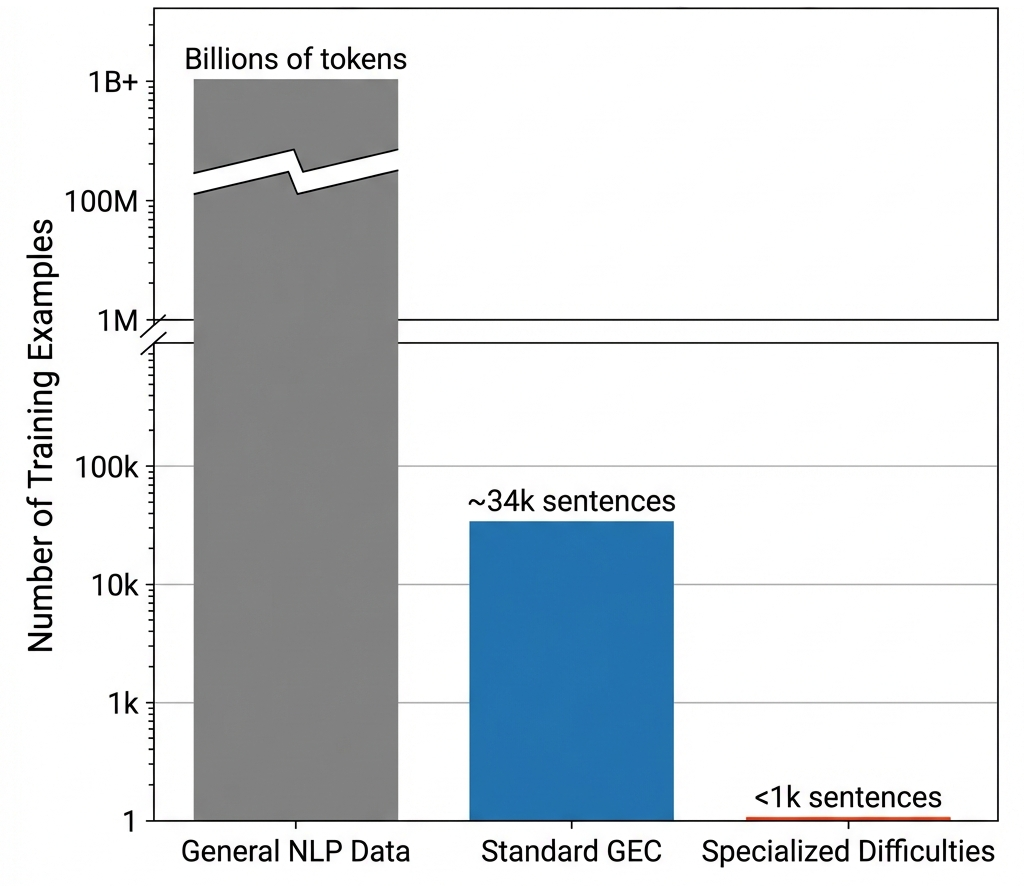
\includegraphics[width=0.7\textwidth]{figures/data_scarcity.png}
\caption{Comparison of training data availability showing the orders-of-magnitude gap between general NLP, standard GEC, and specialized difficulty domains.}
\label{fig:data_scarcity}
\end{figure}

The NUCLE corpus, used in CoNLL-2014, contains approximately 57,000 sentences; the FCE corpus roughly 30,000 sentences; and the combined BEA-2019 training pool approximately 34,000 examples \parencite{Ng2014,Bryant2019,YannakoudakisBriscoeMedlock2011}. These datasets, while valuable, are small relative to general pretraining corpora and concentrated on specific learner populations. For K--12 education, difficulty-specific error patterns, and languages other than English, labeled data is even scarcer \parencite{Joshi2020,Bryant2023GECsurvey}.

\subsection{Rule-based synthetic error generation}
\label{sec:sota_synth_rule}

Rule-based corruption provides a controlled mechanism for generating synthetic training data by systematically transforming correct text into errorful versions. In GEC research, noise injection methods include random character operations (insertions, deletions, substitutions, transpositions), word-level swaps, and rule-based grammatical corruptions \parencite{Lichtarge2020}. These approaches generate large volumes of parallel data but risk producing error distributions that do not match authentic learner behavior.

For difficulty-linked patterns, rule-based generation is more theory-informed. Phonological substitution rules implement systematic voiced/voiceless consonant swaps (e.g., /p/$\leftrightarrow$/b/, /t/$\leftrightarrow$/d/) based on documented confusion patterns in dyslexia research \parencite{ShaywitzShaywitz2005}. Orthographic corruption rules target specific phenomena such as consonant doubling errors, silent letter omissions, and homophone confusions.

\subsection{LLM-based synthetic data generation}
\label{sec:sota_synth_llm}

Large Language Models offer an alternative mechanism for generating synthetic educational data. LLMs produce learner-like text with specific error patterns when prompted, potentially capturing stylistic and contextual properties that rule-based methods miss \parencite{Brown2020,Ouyang2022}. Several approaches exist: (i) direct prompting, where LLMs generate responses ``as if written by a student with specific difficulties''; (ii) controlled generation with conditioning signals to specify target error types; and (iii) hybrid approaches where LLMs generate base responses that are then corrupted using rule-based methods to keep the labels accurate.

Recent studies confirm that LLMs can act as strong error generators and correctors \parencite{CoyneSakaguchi2023,Bryant2023GECsurvey}. Fine-tuning an open LLM (Llama~2) to generate errors has been shown to yield synthetic errors similar to human errors and, when these are used to train correction models, to improve on previous state-of-the-art results for German, Ukrainian, and Estonian \parencite{Luhtaru2024}. LLM-generated synthetic data also carries risks. Generated errors may not match authentic learner distributions, and models may hallucinate implausible patterns. Quality control (human review of samples, comparison against authentic error distributions, and validation of label accuracy) is needed before LLM-generated data is used for training educational systems \parencite{Bryant2023GECsurvey}. These cautions echo wider discussions of the opportunities and challenges of LLMs in education \parencite{Kasneci2023}.

\subsection{Evaluating synthetic data effectiveness}
\label{sec:sota_synth_eval}

The effectiveness of synthetic data depends on alignment between the synthetic distribution and the target deployment population. \textcite{Lichtarge2020} demonstrated that data weighting improves GEC performance by giving more weight to training examples similar to the target distribution. In educational settings, validation implies distribution analysis (comparing error-type frequencies in synthetic and authentic data), transfer evaluation, and generalization checks. The thesis follows these evaluation principles by explicitly comparing models trained with and without synthetic augmentation \parencite{Lichtarge2020,Bryant2023GECsurvey}.

\section{Learning difficulties, profiles, and ethical considerations}
\label{sec:sota_ethics}

The last building block of the thesis is how learning difficulties can be approached computationally without making clinical claims. The subsections below start with computational approaches to learning difficulty detection, move to student profiling and cluster-based analytics, and end with the ethical constraints and non-clinical framing that guide the design of the system.

\subsection{Computational approaches to learning difficulty detection}
\label{sec:sota_ethics_detect}

A growing body of research explores computational methods for detecting indicators of learning difficulties from digital traces. In reading and writing, research has characterized the distribution of errors in text written by learners with dyslexia and contrasted it with that of typically developing peers \parencite{ShaywitzShaywitz2005,RelloBaezaYates2014}. While this research shows that certain error patterns (phonological substitutions, orthographic inconsistencies, and segmentation difficulties) occur more frequently in individuals with dyslexia, it also reports substantial individual variation and overlap between populations. A recent systematic review of machine-learning-based dyslexia screening draws mainly on signals such as electroencephalographic recordings, eye-tracking, and handwriting analysis \parencite{JanKhan2023}, which differ from the typed, text-only setting adopted in this thesis.

In mathematics, research on dyscalculia and math learning difficulties identified characteristic error patterns, including difficulties with number magnitude comparison, procedural bugs in arithmetic, and fraction misconceptions \parencite{VanLehn1990,BrownBurton1978}. These patterns work as proxies or risk indicators, but they do not constitute diagnostic criteria in clinical or educational-psychological terms.

\subsection{Student profiling and cluster-based analytics}
\label{sec:sota_ethics_profiles}

Educational data mining offers methods for aggregating error signals into student profiles. Clustering algorithms (e.g., k-means, hierarchical clustering) group students by similarity in error distributions and can reveal subgroups with distinct difficulty patterns \parencite{BakerYacef2009,RomeroVentura2010EDM}. Knowledge tracing and its neural variants model skill acquisition over time \parencite{CorbettAnderson1995,Piech2015}.

For teacher-facing analytics, profiles have to be interpretable. Clusters should correspond to actionable pedagogical categories, not opaque statistical groupings, and validation against educator intuition and external assessments is necessary \parencite{RomeroVentura2024}. Profile labels must avoid stigmatizing language and should frame patterns as areas for instructional attention and not present them as fixed student attributes.

\subsection{Ethical constraints and non-clinical framing}
\label{sec:sota_ethics_ethical}

The application of AI to detecting learning difficulties raises serious ethical concerns that this thesis addresses directly. First, the framing must be non-clinical. Automated systems cannot and should not provide clinical diagnoses of dyslexia, dyscalculia, or other learning disabilities. Diagnosis requires a full assessment by qualified professionals \parencite{ShaywitzShaywitz2005}. This thesis frames system outputs as \emph{pedagogical indicators} that may warrant further attention, not diagnostic labels.

Second, system outputs are designed for teacher review and interpretation, not for automated decision-making about students \parencite{Woolf2010}.

Third, data protection and privacy need attention. Educational data is sensitive, and more so when it is linked to potential learning difficulties. Processing requires compliance with relevant regulations, above all the General Data Protection Regulation (GDPR) \parencite{EU2016GDPR}, including data minimization, purpose limitation, and appropriate security. In addition, AI systems intended to evaluate learning outcomes, including when these are used to steer the learning process, are classified as high-risk under Annex~III (point~3(b)) of the European Artificial Intelligence Act \parencite{EU2024AIAct}. Although this thesis targets formative, teacher-reviewed indicators rather than grading or admission decisions, this classification reinforces the need for human oversight, transparency, and careful data governance.

Finally, labeling students with difficulty indicators risks stigmatization if misused. System design should use growth-oriented framing and avoid deficit framing. A recent systematic review of fairness, accountability, transparency, and ethics in AI for higher education finds that fairness receives substantially more attention than accountability or transparency \parencite{MemarianDoleck2023}. This supports the emphasis placed here on transparent, teacher-reviewable outputs.

\section{Identified gaps and thesis contribution}
\label{sec:sota_gaps}

The review above points to three gaps in the literature: underrepresented languages and local educational contexts, the limited use of synthetic data for difficulty-linked error patterns, and the scarcity of longitudinal analysis beyond single responses. Each gets its own subsection, together with a statement of how the thesis addresses it. The section closes by positioning the integrated contribution of the thesis with respect to these gaps.

\subsection{Gap 1: Underrepresented languages and local educational contexts}
\label{sec:sota_gap_pt}

The most mature evaluation ecosystems for error-centric educational NLP are centered on a small set of widely used learner corpora and shared tasks \parencite{Ng2014,Bryant2019,BryantFeliceBriscoe2017}. Extending these methods requires aligning label inventories and evaluation protocols with the intended pedagogical use, especially when outputs must be interpretable for teacher review \parencite{Bryant2023GECsurvey,Woolf2010}. The scarcity of resources in specific languages further complicates this, as noted by \textcite{Joshi2020}. Recent studies on Portuguese pursue proficiency assessment \parencite{Akef2026} and general spelling and grammar correction \parencite{Cabral2026}; as far as the reviewed literature shows, they do not target difficulty-linked error patterns in school-age writing.

The thesis responds with formative outputs (error locations and types) that aggregate across tasks and time, and with evaluation grounded in benchmark-informed metrics that are explicitly validated for the local educational context.

\subsection{Gap 2: Limited use of synthetic data for difficulty-linked error patterns}
\label{sec:sota_gap_synth}

While synthetic error generation has been explored in general GEC research, including recent LLM-based approaches \parencite{Luhtaru2024}, its application to difficulty-linked error patterns (those specifically associated with learning difficulties such as dyslexia or dyscalculia) remains underexplored \parencite{Lichtarge2020,Bryant2023GECsurvey}. Existing approaches typically generate generic grammatical errors rather than the systematic phonological, orthographic, and segmentation patterns that research connects to persistent learning difficulties \parencite{ShaywitzShaywitz2005}.

To address this gap, the thesis designs theory-informed, rule-based synthetic data generators that produce error patterns aligned with established taxonomies of learning difficulties \parencite{Bryant2023GECsurvey}; LLM-based generation was considered and, for the reasons given in Section~\ref{sec:method_data_llm}, not adopted.

\subsection{Gap 3: Longitudinal difficulty patterns beyond single responses}
\label{sec:sota_gap_long}

Most benchmark evaluations in error detection and correction focus on sentence-level or essay-level outcomes, while educational practice often requires longitudinal evidence to distinguish episodic mistakes from persistent learning difficulties \parencite{RomeroVentura2024}.

Here the thesis models error recurrence explicitly. Extracted error signals are aggregated over time and analyzed to identify stable profiles of difficulty, informed by educational data mining practices and longitudinal learning perspectives \parencite{BakerYacef2009,RomeroVentura2024}.

\subsection{Integrated thesis contribution and positioning}
\label{sec:sota_contrib}

By integrating error-centric NLP, symbolic mathematical analysis, theory-informed synthetic data, and longitudinal profiling, this thesis positions itself at the intersection of automated assessment and intelligent tutoring. Concretely, it builds on benchmark-driven evaluation practice for error-centric NLP, uses established sequence-labeling architectures for interpretable detection, and grounds feedback design in ITS principles that give priority to difficulty identification and actionable intervention \parencite{DahlmeierNg2012,Ng2014,BryantFeliceBriscoe2017,ReiYannakoudakis2016,MaHovy2016,Woolf2010}.

The intended outcome is a text-based system that (i) detects and classifies error patterns linked to learning difficulties in typed student responses, (ii) uses synthetic data to address data scarcity, and (iii) surfaces persistent difficulty patterns as interpretable, non-clinical profiles to support pedagogical decision-making \parencite{Bryant2023GECsurvey,RomeroVentura2024}.

% Chapter 3

\chapter{Methods, Data, and Tools} % Main chapter title
\label{chap:Chapter3} % For referencing the chapter elsewhere, use \ref{chap:Chapter3}

%----------------------------------------------------------------------------------------

This chapter describes how error patterns linked to learning difficulties are detected in typed student responses. Section~\ref{sec:method_tax} formalizes the error taxonomies for the linguistic and mathematical domains, and Section~\ref{sec:method_data} covers the data strategy and the decisions behind it. The detection and profiling methods follow in Section~\ref{sec:method_models}, and the evaluation framework in Section~\ref{sec:method_eval}. Section~\ref{sec:method_poc} summarizes the initial proof of concept, whose limitations motivated the final design. Alternatives that were considered and rejected are documented together with the reasons for rejecting them, because several of those decisions (language of experimentation, data sources, synthetic-generation method) shaped the results reported in Chapter~\ref{chap:Chapter5}.

\section{Error Taxonomies}
\label{sec:method_tax}

Automated error detection needs a formal taxonomy that defines the target error types, gives operational criteria for labeling, and links observable patterns to pedagogically meaningful categories. The taxonomies adopted here draw on educational psychology and learning-difficulty research (Figure~\ref{fig:error_taxonomy}). The linguistic categories come first, then the mathematical ones, and the label scheme used for annotation closes the section.

\begin{figure}[ht]
\centering
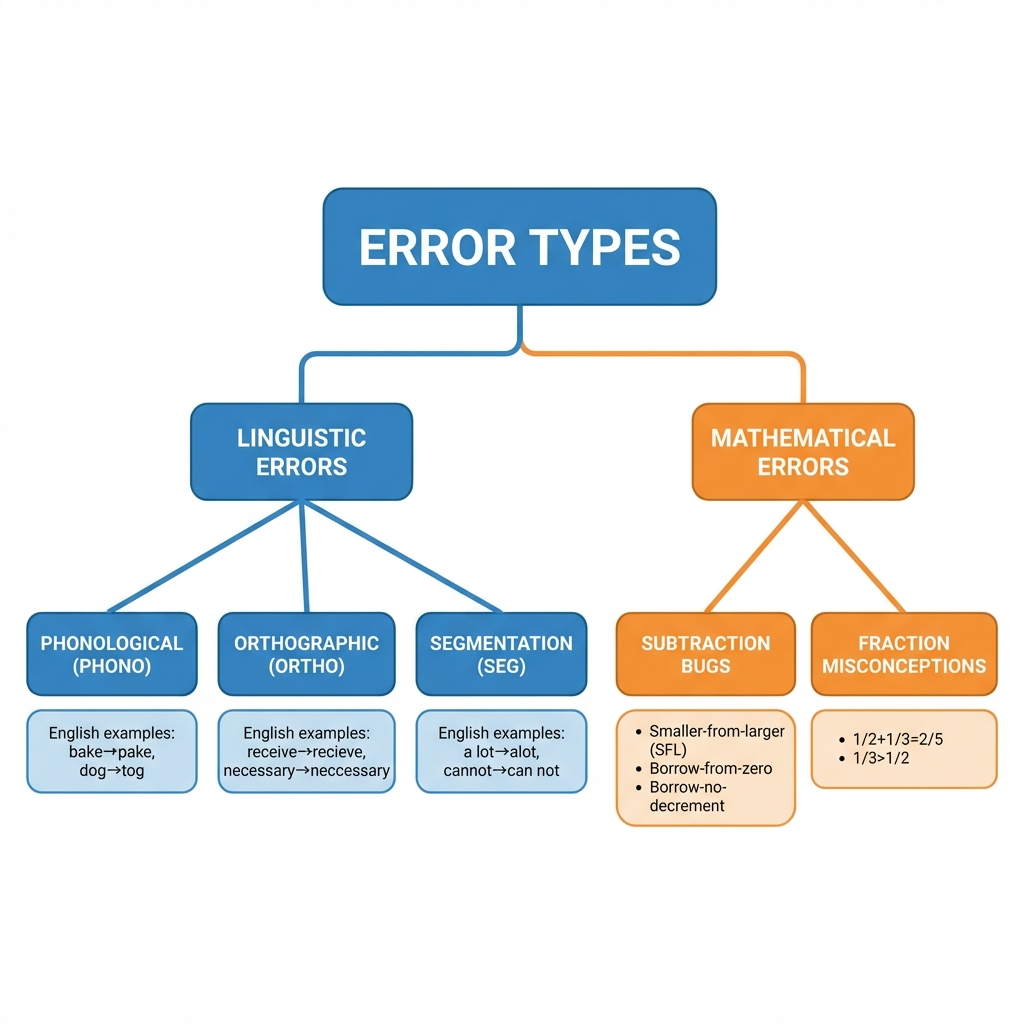
\includegraphics[width=0.9\textwidth]{figures/error_taxonomy.png}
\caption{Hierarchical error taxonomy showing linguistic and mathematical error categories with examples.}
\label{fig:error_taxonomy}
\end{figure}

\subsection{Linguistic Error Categories}
\label{sec:method_tax_ling}

For linguistic errors in typed student text, the taxonomy targets patterns associated with persistent learning difficulties, not general grammatical or typographical errors. Three primary categories are defined.

\textbf{Phonological Errors (ERR-PHONO).} These errors are commonly associated in the learning-difficulty literature with difficulty in phoneme-grapheme conversion, as described in accounts of phonological dysorthography. Observable patterns include:
\begin{itemize}
    \item Voicing substitutions are systematic confusions between voiced and voiceless consonants (e.g., /p/$\leftrightarrow$/b/, /t/$\leftrightarrow$/d/, /f/$\leftrightarrow$/v/, /k/$\leftrightarrow$/g/). Example: ``bato'' for ``pato'', ``gola'' for ``cola''.
    \item Syllable inversions reorder phonemes within words. Example: ``parto'' for ``prato'', ``trota'' for ``torta''.
\end{itemize}

\textbf{Orthographic Errors (ERR-ORTHO).} These errors are commonly associated with difficulty in visual-orthographic memory, where the student struggles to recall correct spellings despite intact phonological processing. Observable patterns include:
\begin{itemize}
    \item Contextual rule violations are errors in context-dependent spelling rules (e.g., ``s'' vs. ``ss'' vs. ``ç'' in Portuguese; ``c'' vs. ``k'' in English). Example: ``caza'' for ``casa''.
    \item Homophone confusions substitute words that sound identical but differ in spelling. Example: ``há'' vs. ``à'', ``their'' vs. ``there'' vs. ``they're''.
\end{itemize}

\textbf{Segmentation Errors (ERR-SEG).} These errors reflect difficulty in word boundary perception. Observable patterns include:
\begin{itemize}
    \item Hyposegmentation is the incorrect joining of words. Example: ``derrepente'' for ``de repente'', ``alot'' for ``a lot''.
    \item Hypersegmentation is the incorrect splitting of words. Example: ``em baixo'' for ``embaixo'', ``to gether'' for ``together''.
\end{itemize}

Classification also depends on the semantic context of the error. For example, ``bato'' is a valid Portuguese word (``I beat''), so detecting it as a phonological error for ``pato'' (``duck'') requires analyzing the surrounding sentence context. This motivates the use of contextual language models (Section~\ref{sec:method_models_ling}).

The taxonomy is operational: each category is defined by an observable surface relationship between the written form and its target (phonetic faithfulness, boundary structure, rule- or homophone-based substitution; the mapping rules are given in Section~\ref{sec:impl_ling_taxmap}). The associations with underlying processing difficulties stated above are motivational, drawn from the learning-difficulty literature; they are not constructs the system measures. The taxonomy itself is language-general; the three categories describe error-production mechanisms, not properties of any particular orthography. The implementation and evaluation in this thesis are English-language, for data-availability reasons discussed in Section~\ref{sec:method_data_sources}; Portuguese examples are retained above because the taxonomy was originally motivated by the Portuguese school context, and Portuguese support is the most valuable direction for future work (Chapter~6).

\subsection{Mathematical Error Categories}
\label{sec:method_tax_math}

For mathematical errors in typed numeric responses, the taxonomy targets systematic procedural misconceptions, not computational slips. Two primary categories are defined, following the ``malrule'' tradition in cognitive modeling \parencite{VanLehn1990,BrownBurton1978}:

\textbf{Subtraction Procedural Bugs (ERR-SUB).} Systematic errors in multi-digit subtraction that reflect incorrect procedural rules, not careless mistakes. Specific bugs include:
\begin{itemize}
    \item In the smaller-from-larger bug (SFL), the student always subtracts the smaller digit from the larger, ignoring column position. Example: $43 - 17 = 34$ (computing $7-3=4$ and $4-1=3$).
    \item In borrow-from-zero, borrowing is handled incorrectly when a zero is present. Example: $302 - 158 = 254$ (treating the zero as 10 without borrowing from the hundreds).
    \item In borrow-no-decrement, the student borrows to the ones column but fails to decrement the tens column. Example: $52 - 27 = 35$ (computing $12-7=5$ but then $5-2=3$).
\end{itemize}

\textbf{Fraction Misconceptions (ERR-FRAC).} Conceptual errors in fraction operations rooted in ``whole-number bias'', the tendency to treat fraction components as independent integers. Specific misconceptions include:
\begin{itemize}
    \item Independent numerator-denominator addition means adding fractions by adding numerators and denominators separately. Example: $\frac{1}{2} + \frac{1}{3} = \frac{2}{5}$.
    \item Magnitude comparison by component means comparing fractions by comparing numerators or denominators independently. Example: claiming $\frac{1}{5} > \frac{1}{3}$ because $5 > 3$.
\end{itemize}

In the buggy-procedure tradition these error patterns are regarded as diagnostically informative, since they reveal a systematically applied incorrect rule rather than an isolated slip, which motivates their early identification \parencite{VanLehn1990}.

\subsection{Label Scheme and Annotation Guidelines}
\label{sec:method_tax_labels}

For linguistic errors, the annotation scheme adopts a token-level or span-level labeling format compatible with sequence-labeling models. The BIO (Begin-Inside-Outside) tagging scheme applies:
\begin{itemize}
    \item \texttt{O}: Token is correct (outside any error span).
    \item \texttt{B-PHONO}: Beginning of a phonological error span.
    \item \texttt{I-PHONO}: Inside a phonological error span.
    \item Similarly for \texttt{B-ORTHO}/\texttt{I-ORTHO} and \texttt{B-SEG}/\texttt{I-SEG}.
\end{itemize}

For mathematical errors, each student response (problem-answer pair) receives a categorical label from the set: \{\texttt{CORRECT}, \texttt{SFL}, \texttt{BORROW\_ZERO}, \texttt{BORROW\_NO\_DEC}, \texttt{FRAC\_ADD}, \texttt{FRAC\_COMPARE}, \texttt{OTHER\_ERROR}\}.

\section{Data Strategy}
\label{sec:method_data}

Data scarcity is the main methodological challenge of this thesis. Corpora of student responses annotated with difficulty-linked error types, for K--12 populations, with per-student longitudinal structure, are almost nonexistent in public form, for the same privacy and ethics reasons (GDPR, data about minors) that make collecting them hard. The thesis treats this as the problem statement behind hypothesis H2, namely whether synthetic data can compensate when real data cannot be obtained at scale. The subsections below document the data sourcing decisions, including the sources that were considered and rejected.

\subsection{Data Source Selection}
\label{sec:method_data_sources}

On language, the project was initially oriented toward Portuguese, the natural deployment context. The best available Portuguese error-annotated resource, the COPLE2 learner corpus \parencite{Mendes2016}, was examined and rejected as a primary source because of a population mismatch. COPLE2 documents adult foreign learners of Portuguese, whose error distribution (interference from the mother tongue, morphosyntax of a second language) differs fundamentally from that of native-speaker children with learning difficulties. Since no Portuguese child-population error corpus was available, and the thesis's research questions do not depend on any particular language, experimentation moved to English, where substantially larger error-annotated corpora exist. This trade of deployment realism for data availability and statistical power is revisited in the limitations (Chapter~5) and future work (Chapter~6).

For real linguistic data, candidate English corpora were assessed against three criteria: error annotations at span level (corrected text alone was not enough), a license obtainable within the project's timeline, and a machine-readable format with an existing parsing ecosystem. The outcome for each corpus follows.
\begin{itemize}
    \item BEA-2019 W\&I+LOCNESS \parencite{Bryant2019} was adopted. It provides gold ERRANT/M2 span annotations, is free for non-commercial research, and can be downloaded directly.
    \item CLC FCE v2.1 \parencite{YannakoudakisBriscoeMedlock2011} was also adopted; it has the same M2 format and license class. It was initially catalogued as requiring signed license paperwork and deferred; a later check found the BEA-2019 release of FCE is directly downloadable, and it was integrated, growing the real training pool by a factor of 2.7 (Chapter~5).
    \item NUCLE/CoNLL-2014 was rejected. It requires signed institutional license agreements with turnaround incompatible with the project timeline, and adds no annotation type the adopted corpora lack.
    \item Lang-8/cLang-8 ($\sim$2.4M sentence pairs) was deferred. It requires a registration process with manual approval, and was identified as the natural scale-up path if the adopted corpora proved insufficient, which the results of Chapter~5 did not indicate.
    \item The Holbrook corpus \parencite{Holbrook1964,Mitton1985} contains writings of 19 schoolchildren with severe literacy difficulties and was adopted for evaluation only. It is the only located public English corpus from (approximately) the target population. With 531 usable sentences it is far too small to train on, but it suits the measurement of domain shift from the adult-learner training corpora to struggling child writers. The Spanish DysList resource \parencite{RelloBaezaYates2014} confirms that dyslexic-error corpora exist for other languages but offers no English data.
\end{itemize}

For mathematics, the original plan used DeepMind's \texttt{mathematics\_dataset} generator as the source of correct base problems for malrule injection. It was discarded during implementation because the package is unmaintained and incompatible with current versions of its own dependencies. The needed problem classes (multi-digit subtraction, fraction pairs) are trivially generatable, so a self-written generator replaced it; a heavyweight external dependency was not worth its maintenance risk for 50 lines of controlled generation code. The MaE dataset of expert-validated algebra misconceptions (MIT license) was retained as reference material for future extension beyond arithmetic. The ASSISTments 2009--10 dataset \parencite{Feng2009Assistments} was examined as a source of math error labels and found unsuitable for that purpose. It records correctness, attempts, and hints, but not \emph{which} procedural bug produced a wrong answer. Those same behavioral signals make it valuable for the profiling module (below), where it was adopted instead.

For profiling, no public dataset offers longitudinal, per-student, difficulty-labeled responses (the GDPR/minors constraint above binds hardest here). The strategy therefore has three parts: (i) a simulator with known ground-truth archetypes, testing whether they can be recovered; (ii) the Holbrook corpus reused at the student level (per-child error distributions), testing whether archetype-like structure exists in real struggling writers; and (iii) ASSISTments (525{,}534 responses, 4{,}217 students), testing whether behavioral profiles are stable per-student traits over real longitudinal histories. None of the three alone would support H3, so the design uses separate data for recoverability, realism, and stability.

\subsection{Rule-Based Synthetic Data Generation}
\label{sec:method_data_rule}

Rule-based generators provide controlled synthetic data with guaranteed label accuracy, because the corruption is injected programmatically and the BIO span labels are therefore correct by construction. Starting from correct sentences, corruption rules inject specific error types:
\begin{itemize}
    \item Phonological errors come from probabilistic substitution of confusable consonant pairs (p/b, t/d, f/v, k/g) and phonetically-faithful respellings, based on documented confusion patterns.
    \item Orthographic errors come from substitution of frequently confused grapheme patterns and homophone swaps.
    \item Segmentation errors come from word fusion (removing spaces) or word splitting (inserting spaces at plausible boundaries).
\end{itemize}

Correct base sentences are drawn from a public Wikipedia-derived sentence corpus, filtered to 5--18 words and plain punctuation ($\sim$600{,}000 sentences). The size of the base pool came from a failure. The first implementation used 20 hand-written template sentences, and the resulting evaluation scores turned out to measure template memorization, not generalization (Chapters~4 and~5 document this failure and its diagnosis). For mathematics, transformation rules apply each malrule to generated problems, recording correct answer, malrule answer, and label; problems where two malrules produce identical answers are filtered out as formally ambiguous (Chapter~4).

\subsection{LLM-Based Synthetic Data Generation: Considered, Not Adopted}
\label{sec:method_data_llm}

Large Language Models were considered as a second synthetic-data source, generating more naturalistic student errors via few-shot prompting. This path was not adopted in the final system, for three reasons weighed against the properties of the rule-based generator:
\begin{enumerate}
    \item Rule-based corruption yields span labels that are correct by construction, whereas LLM-generated errors require post-hoc verification of both the error's type and its exact span. That reintroduces, at scale, the annotation cost the synthetic strategy exists to avoid.
    \item The final training set uses $10^6$ synthetic sentences. Generating at that scale through commercial LLM APIs would have a real cost, while the rule-based generator is free and fast.
    \item The taxonomy's three categories are surface-realizable by rules (substitutions, splits, merges); the added naturalness of LLM text plausibly matters more for error types this thesis does not target (discourse-level, semantic).
\end{enumerate}
LLM generation remains attractive for future work where rules are weakest, that is, generating errors with the distributional signature of a specific population (e.g., mimicking the Holbrook error mix identified in Chapter~5) instead of uniform corruption.

\subsection{Data Splits and Validation}
\label{sec:method_data_splits}

The synthetic and real pools are partitioned into training and evaluation splits (90/10). To assess the effect of synthetic data (H2), experiments compare models trained on synthetic data only, real data only, and combined data. Because the curriculum stages are chained (each stage continues from the previous checkpoint; Section~\ref{sec:impl_ling_training}), the real-only comparison point for H2 is a separate model trained on the real pool alone, from the pretrained encoder, with no synthetic stage (Section~\ref{sec:eval_ling_scratch}). One protocol rule, learned the hard way (Chapter~5), is that all claims about real-data performance are measured on all-real evaluation sets, and two additional benchmarks (FCE test; Holbrook) are held out from training entirely.

\section{Proposed Methods}
\label{sec:method_models}

The methods below cover error detection, linguistic and mathematical, and the aggregation of detected errors into student difficulty profiles.

\subsection{Linguistic Error Detection: NLP Sequence Labeling}
\label{sec:method_models_ling}

Linguistic error detection is framed as a sequence-labeling problem, where each token in the input text is assigned an error-type label (or \texttt{O} for correct) \parencite{MaHovy2016,ReiYannakoudakis2016}. This framing was chosen over the sequence-to-sequence formulation dominant in grammatical error correction. The thesis needs to detect and categorize error spans, not rewrite the text, and tagging formulations are cheaper to train and directly interpretable per token \parencite{Omelianchuk2020GECToR}.

The architecture is a pretrained Transformer encoder fine-tuned for token classification, with three parts.
\begin{itemize}
    \item The encoder is a pretrained language model; candidates included BERT, RoBERTa, XLM-RoBERTa (for future multilingual work) and DeBERTa-v3. The final selection (DeBERTa-v3-base) and its rationale are given in Chapter~\ref{chap:Chapter4}.
    \item The classification head is a linear layer mapping each token's contextual embedding to the label space (\texttt{O}, \texttt{B-PHONO}, \texttt{I-PHONO}, \texttt{B-ORTHO}, \texttt{I-ORTHO}, \texttt{B-SEG}, \texttt{I-SEG}).
    \item Training uses a token-level classification loss. The label distribution is severely imbalanced (most tokens are correct), and the choice of loss function turned out to be one of the hardest implementation problems of the thesis; Chapter~\ref{chap:Chapter4} documents the full progression (plain cross-entropy, weighted variants, focal loss) with the observed failure of each intermediate step.
\end{itemize}

Pretrained Transformers use subword tokenization, which typically splits misspelled words differently from correct words. Error labels are assigned to the first subword of each token, with subsequent subwords receiving a continuation label or being ignored during evaluation.

Contextual models can distinguish legitimate words from contextual errors. For example, ``bato'' is correctly predicted as an error in ``O bato nada'' (intended: ``O pato nada'') but not in ``Eu bato à porta'' (correct usage).

\subsection{Mathematical Error Detection: Symbolic and ML Methods}
\label{sec:method_models_math}

Mathematical error detection uses the structured nature of arithmetic problems and deliberately implements two contrasting methods, since their comparison is itself a research question (Q3).

The symbolic method is malrule simulation. For each known misconception (SFL, borrow-from-zero, etc.), a procedural simulation computes what result the student would produce if applying that malrule. The student's actual response is compared against the correct answer and each malrule's predicted answer; an exact match assigns the label. This method is exact and interpretable by construction and, by the same construction, intolerant to any deviation from the modeled procedure.

The second method is a feature-based ML classifier: a gradient-boosted decision tree classifier over hand-built numeric features of the (problem, answer) pair, trained on generator output. The initial plan called for this classifier only as an optional disambiguator; it was promoted to a co-equal method during implementation, both because the thesis's research questions explicitly compare symbolic and ML approaches and because early experiments showed the two methods fail in complementary ways (exactness versus robustness, quantified in Chapter~5).

\subsection{Active Screening vs.\ Passive Monitoring}
\label{sec:method_models_screening}

The system distinguishes two acquisition regimes for linguistic errors, routed to different detection methods.

\textbf{Passive monitoring (open world).} In free writing, the intended words are unknown; detecting an error requires inferring both that a span is wrong and what was meant. Only a learned contextual model can solve this inference problem. It is where the neural sequence labeler operates, and where its training-population dependence matters.

\textbf{Active screening (closed world).} In a designed worksheet item (dictation of a target word; an arithmetic problem), the correct answer is known in advance. Error classification then reduces to comparing the written form against the known target through the same deterministic taxonomy logic used to build the corpora, with no model inference and no training-population dependence. The cost is coverage, since screening only observes the items it poses.

The closed-world regime has a second advantage, \emph{item selection}. Each screening item is chosen to maximize the diagnostic information of the error it may elicit: irregularly-spelled but phonetically recoverable words isolate the orthographic-memory profile; short regular words isolate phoneme-grapheme conversion; compounds isolate word segmentation; and arithmetic items are admitted only if every modeled malrule yields a distinct answer (the distinguishability policy of Chapter~5). This is the same principle as classical diagnostic test design, applied programmatically. The two regimes are complementary by design. Screening is intended to yield high-information signal from one or two worksheets and, having no trained component, does not depend on any training population (it does depend on the item bank and on the mapper's rules); monitoring accumulates broad-coverage signal over time.

\subsection{Student Difficulty Profiling: Clustering and Aggregation}
\label{sec:method_models_profile}

Error detection produces per-response labels. To identify persistent difficulty patterns, errors are aggregated across multiple responses per student and analyzed for stability.

For each student, an error profile vector is constructed from the proportion of each error type among the student's errors, the overall error rate, and the temporal trend of errors across sessions. The overall rate is included alongside the proportions because proportion-only vectors are provably blind to profiles that differ in error frequency but not error mix; Chapter~4 documents this defect, which was found empirically in simulation.

Clustering uses KMeans (fixed $k$, swept by silhouette) and HDBSCAN \parencite{Campello2013HDBSCAN} (no fixed $k$, native outlier handling, which matters because students with atypical profiles are exactly the interesting cases in this application). Hierarchical clustering and plain DBSCAN were considered; HDBSCAN subsumes the practical advantages of both for this use case.

Cluster centroids are examined to identify the characteristic error pattern of each group (e.g., ``phonological-dominant''). Interpretability is assessed by centroid inspection against the taxonomy; validation with practicing educators is planned as part of the future school pilot (Chapter~6), not claimed here. Throughout the thesis, ``difficulty profile'' denotes such a statistical profile over observable error patterns; it is not a measurement of an underlying cognitive or clinical construct (Section~\ref{sec:eval_discuss_threats}).

Where longitudinal data is available, error recurrence is analyzed: a profile is considered stable if the same error types persist across multiple sessions, distinguishing persistent difficulties from episodic mistakes.

\section{Evaluation Framework}
\label{sec:method_eval}

Each component of the system is evaluated with the metrics and protocols specified in the subsections below.

\subsection{Error Detection Metrics}
\label{sec:method_eval_detect}

For linguistic error detection (sequence labeling), evaluation uses span-level metrics computed with seqeval:
\begin{itemize}
    \item Precision is the fraction of predicted error spans that exactly match gold spans (boundary and type).
    \item Recall is the fraction of gold error spans that are exactly predicted.
    \item The $F_1$-score is the harmonic mean of precision and recall.
\end{itemize}

Span-level scoring with exact boundaries is deliberately strict; it understates partial credit but cannot be gamed by over-flagging. Metrics are reported per benchmark; per-error-type breakdowns and predicted-tag distributions are inspected diagnostically (a model collapsing to a single class is visible in the distribution but not in aggregate $F_1$).

For mathematical error detection, evaluation uses classification metrics: accuracy, macro-$F_1$ over error classes, and confusion analysis for systematic misclassifications.

\subsection{Clustering Metrics}
\label{sec:method_eval_cluster}

For student difficulty profiling, clustering quality is assessed using:
\begin{itemize}
    \item The silhouette coefficient \parencite{Rousseeuw1987} measures cluster cohesion and separation, and is used for internal quality and $k$ selection.
    \item The Adjusted Rand Index \parencite{HubertArabie1985} measures agreement with ground truth where it exists (simulation), and agreement between independent re-clusterings where it does not (split-half stability on real data).
    \item The Davies--Bouldin index \parencite{DaviesBouldin1979} is a secondary internal-quality check.
\end{itemize}

\subsection{Synthetic vs. Real Data Comparison}
\label{sec:method_eval_synth}

To assess the effectiveness of synthetic data (H2), experiments compare performance on held-out real test data when training on synthetic-only, real-only (from scratch), and combined data. Two protocol rules apply, both introduced after evaluation-design failures documented in Chapter~5. Evaluation splits must not share base material with training data (the template-memorization incident), and mixed-composition evaluation sets must not be used for real-data claims (the synthetic-dominated-eval incident).

\section{Tools and Implementation}
\label{sec:method_tools}

The implementation uses Python (3.10--3.12); PyTorch and Hugging Face Transformers for the neural model; ERRANT's M2 format and parsing conventions \parencite{BryantFeliceBriscoe2017} for real GEC data; seqeval for span-level scoring; scikit-learn \parencite{Pedregosa2011} for the gradient-boosted classifier, clustering, and metrics; jellyfish (Metaphone \parencite{Philips1990}) for phonetic matching in the taxonomy mapper; a purpose-built European Portuguese grapheme-to-phoneme comparator for the Portuguese screening instantiation (Chapter~4); and Flask with SQLite for the pilot prototype (Chapter~4). Sentence-BERT and \texttt{pyspellchecker} appear only in the proof of concept (Section~\ref{sec:method_poc}). The final system lives in the \texttt{System} directory of the project repository; the POC is preserved separately under \texttt{Experimentation}.

\section{Initial Proof of Concept}
\label{sec:method_poc}

Before the full implementation, an initial Proof of Concept (POC) was developed to validate the feasibility of automated error pattern detection. The POC architecture and results are summarized below, together with the reasons its approach was not carried forward as the core of the final system.

\subsection{POC Architecture}
\label{sec:method_poc_arch}

The POC implements a heuristic-based detection pipeline.

Preprocessing consists of normalization (lowercase, whitespace cleaning) and tokenization of the input text (student answer and reference answer).

Feature extraction then computes three parallel feature streams:
\begin{itemize}
    \item For semantic similarity, Sentence-BERT embeddings (model: \texttt{all-MiniLM-L6-v2}) are computed for both reference and student answers, and cosine similarity is calculated.
    \item For keyword analysis, keywords are extracted from the reference answer, and coverage (fraction of keywords present in student answer) is computed.
    \item For linguistic analysis, spelling errors are counted using \texttt{pyspellchecker}.
\end{itemize}

The heuristic detector is a priority-based decision tree that classifies each answer:
\begin{enumerate}
    \item If semantic similarity $\geq 0.75$ and keyword coverage $\geq 50\%$: classify as \texttt{correct}.
    \item If word count $< 5$: flag as \texttt{vague\_answer}.
    \item If spelling errors $\geq 3$: flag as \texttt{linguistic\_error}.
    \item If semantic similarity $< 0.55$: flag as \texttt{conceptual\_error}.
    \item If keyword coverage $< 40\%$: flag as \texttt{missing\_key\_concepts}.
    \item If no issues detected: classify as \texttt{correct}.
\end{enumerate}

The system selects the highest-confidence issue and generates a human-readable explanation.

\subsection{POC Results}
\label{sec:method_poc_results}

The POC was evaluated on a synthetic dataset of 42 English student answers across three science questions (photosynthesis, water cycle, mitosis/meiosis). Error labels were manually assigned.

Performance was as follows.
\begin{itemize}
    \item Overall accuracy: 66.7\% (28/42 correct predictions)
    \item Linguistic errors: 100\% precision, 100\% recall
    \item Vague answers: 100\% precision, 100\% recall
    \item Conceptual errors: 9\% recall (frequently confused with \texttt{missing\_key\_concepts})
\end{itemize}

\subsection{From POC to Full System: What Was Kept and What Was Replaced}
\label{sec:method_poc_future}

The POC validated the core premise that error patterns, as well as correctness, are automatically detectable. Four of its properties, however, disqualified its approach as the core of the final system, and each drove a concrete design decision:

\begin{itemize}
    \item Response-level flags cannot support the taxonomy. The POC classifies whole answers, but the difficulty taxonomy requires knowing which words are wrong and how. This motivated the token-level sequence-labeling formulation (Section~\ref{sec:method_models_ling}).
    \item A spell-checker cannot separate PHONO from ORTHO from SEG. \texttt{pyspellchecker} counts out-of-vocabulary words, whereas the taxonomy's categories depend on the relationship between the misspelling and its target (phonetic faithfulness, boundary structure). This motivated the taxonomy mapper and the learned model.
    \item Fixed thresholds do not generalize. The POC's similarity cut-offs were tuned to 42 examples and its conceptual-vs-missing confusion (9\% recall) showed heuristics saturating. This motivated learned models trained on orders of magnitude more data.
    \item Single-response classification cannot see persistence. Difficulty is a longitudinal construct, and the POC has no notion of a student. This motivated the profiling module.
\end{itemize}

The POC's conceptual/missing-concepts error categories (science-content errors) were deliberately dropped: they concern subject-matter knowledge, not the difficulty-linked mechanical patterns this thesis targets. The POC code is preserved under \texttt{Experimentation} as a baseline and historical record.

\section{Summary}
\label{sec:method_summary}

This chapter covered the following.
\begin{enumerate}
    \item Error taxonomies for linguistic (phonological, orthographic, segmentation) and mathematical (subtraction bugs, fraction misconceptions) errors, grounded in learning-difficulty research.
    \item A data strategy built around documented sourcing decisions: English over Portuguese (population-mismatch of the available Portuguese corpus), BEA-2019+FCE as real training data, Holbrook as a target-population evaluation benchmark, rule-based synthetic generation at the million-sentence scale (LLM generation considered and rejected with stated reasons), and a three-way profiling evidence design (simulation, real archetypes, real stability).
    \item Detection methods: NLP sequence labeling for linguistic errors, and two deliberately contrasted mathematical methods (symbolic simulation and a gradient-boosted classifier).
    \item Profiling methods: clustering of per-student error vectors, with explicit attention to feature-representation limits and outlier handling.
    \item An initial POC (66.7\% accuracy, heuristic) whose specific failure modes (response-level granularity, undifferentiated spelling detection, threshold brittleness, no longitudinal view) directly motivated the design decisions of the final system.
\end{enumerate}

The following chapters present the implementation and its engineering decisions (Chapter~4), experimental results (Chapter~5), and conclusions (Chapter~6).

% Chapter 4

\chapter{System Architecture and Implementation} % Main chapter title
\label{chap:Chapter4} % For referencing the chapter elsewhere, use \ref{chap:Chapter4}

%----------------------------------------------------------------------------------------

This chapter presents the architecture and implementation of the error detection and student profiling system. It describes the overall system design (Section~\ref{sec:impl_arch}), the linguistic error detection module (Section~\ref{sec:impl_ling}), the mathematical error detection module (Section~\ref{sec:impl_math}), and the student profiling module (Section~\ref{sec:impl_profile}). Section~\ref{sec:impl_lessons} documents the main engineering problems encountered during implementation and how they were diagnosed and resolved; these are reported deliberately, since several of them (numerical instability, class-imbalance collapse, evaluation-set composition) are failure modes that any practical deployment of a similar system would face.

\section{System Overview}
\label{sec:impl_arch}

Before the individual modules are described, this section lays out the system as a whole: the modular architecture and the processing pipeline that connects the linguistic, mathematical and profiling components, and then the technology stack used to implement them.

\subsection{High-Level Architecture}
\label{sec:impl_arch_overview}

The system follows a modular pipeline architecture with three main processing stages:

\begin{enumerate}
    \item The input stage ingests student responses (typed text or numeric answers) and routes each one to the appropriate detection module based on content type.
    \item The error detection stage passes each response to a specialized module, which analyzes it for linguistic errors (neural sequence labeling) or mathematical errors (symbolic malrule matching and a feature-based classifier) and produces structured, per-response error annotations.
    \item The profiling and aggregation stage combines the detected error labels across responses and sessions into per-student difficulty profiles, which are then grouped by unsupervised clustering.
\end{enumerate}

The architecture replaces the proof of concept's response-level heuristic pipeline entirely; the specific POC failure modes that drove this replacement are documented in Section~\ref{sec:method_poc_future}. The modules are intentionally decoupled: the profiling module consumes only the output labels of the two detection modules (error-type counts per response), never their internal representations. This separation means each detection module can be improved or replaced independently, and it makes the profiling module's input format identical whether labels come from the neural linguistic model, the symbolic math detector, or (in a validation setting) from gold annotations.

\begin{figure}[ht]
\centering
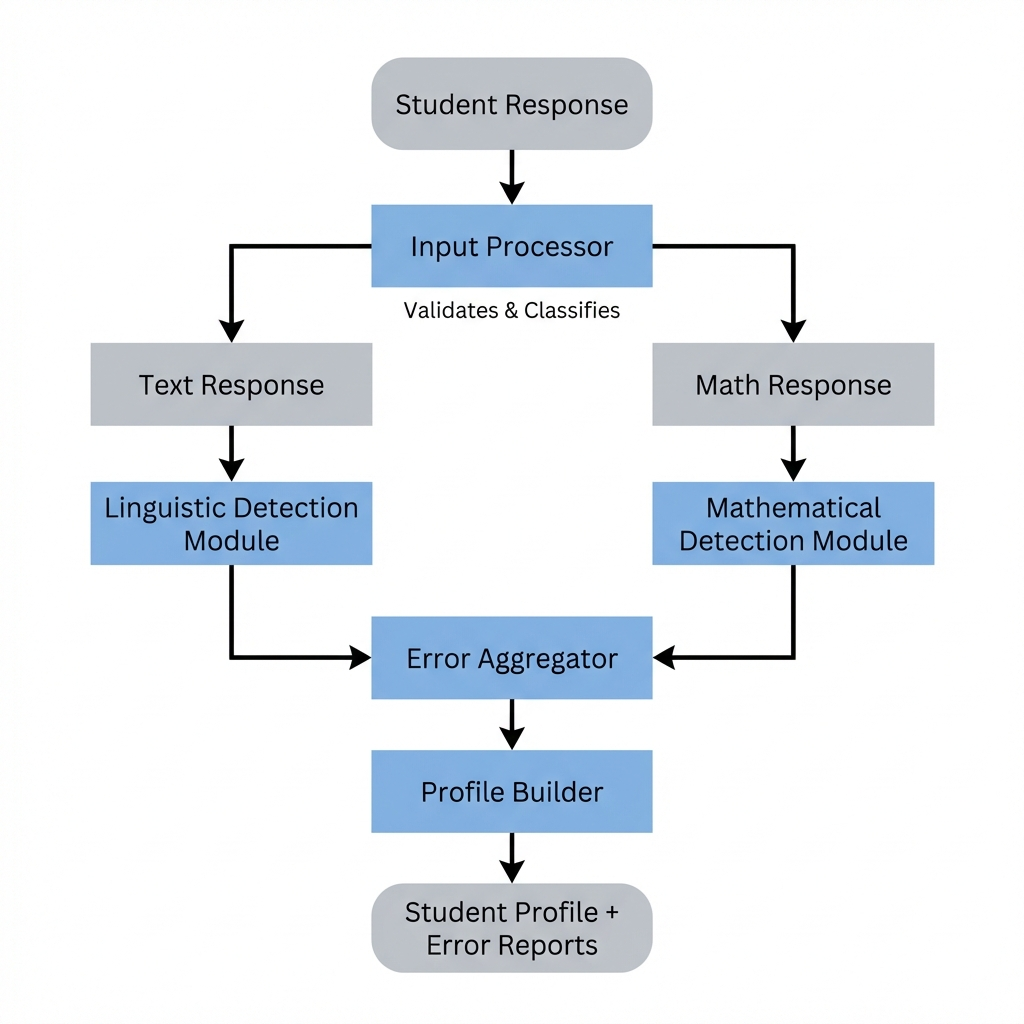
\includegraphics[width=0.85\textwidth]{figures/dataflow.png}
\caption{System data flow from student response to difficulty profile.}
\label{fig:dataflow}
\end{figure}

\subsection{Technology Stack}
\label{sec:impl_arch_stack}

The implementation uses Python (3.10--3.12), PyTorch and Hugging Face Transformers for the neural linguistic model, scikit-learn \parencite{Pedregosa2011} for the classical classifiers and clustering, and the ERRANT toolkit's M2 annotation format \parencite{BryantFeliceBriscoe2017} as the interchange format for real grammatical-error data. Phonetic matching uses the Metaphone algorithm \parencite{Philips1990} via the \texttt{jellyfish} library. Neural training was performed on a single consumer GPU (NVIDIA RTX 5070, 12\,GB VRAM); all other components run on CPU. All datasets, trained models, and experiment outputs are serialized as JSON or CSV for reproducibility.

\section{Linguistic Error Detection Module}
\label{sec:impl_ling}

The linguistic module identifies phonological (\texttt{PHONO}), orthographic (\texttt{ORTHO}), and segmentation (\texttt{SEG}) error spans in typed student text (taxonomy defined in Section~\ref{sec:method_tax_ling}), formulated as token-level sequence labeling with a BIO scheme over seven labels (\texttt{O} plus \texttt{B-}/\texttt{I-} variants of the three categories).

\subsection{Taxonomy Mapping Layer}
\label{sec:impl_ling_taxmap}

Public grammatical error correction (GEC) corpora annotate errors with ERRANT's generic type system (e.g., \texttt{R:SPELL}, \texttt{R:ORTH}), not with this thesis's difficulty-oriented categories. A deterministic mapping layer translates ERRANT-annotated edits into the thesis taxonomy:

\begin{itemize}
    \item An edit whose original and corrected strings contain the same letters grouped into a different number of space-separated tokens is mapped to segmentation (\texttt{ERR-SEG}), e.g., \emph{some times} $\rightarrow$ \emph{sometimes}. Edge punctuation is stripped before comparison, so sentence-boundary fixes (e.g., \emph{we} $\rightarrow$ \emph{. We}) are correctly excluded.
    \item \texttt{R:SPELL} edits are split into phonological and orthographic misspellings by phonetic faithfulness. If the misspelling and its correction share a Metaphone code, the misspelling preserves the word's sound (\texttt{ERR-PHONO}, e.g., \emph{wach} $\rightarrow$ \emph{watch}); otherwise it is treated as a visual/rule-memory slip (\texttt{ERR-ORTHO}).
    \item Homophone confusions between two correctly spelled words (\emph{their}/\emph{there}, \emph{to}/\emph{too}) are matched against a curated closed-class lexicon and mapped to \texttt{ERR-ORTHO}, following the taxonomy in Chapter~3.
    \item All other edits (grammar, word choice, punctuation) are out of scope and mapped to \texttt{OTHER}, leaving their tokens labeled \texttt{O}.
\end{itemize}

In practice, this mapping could not be designed reliably against toy examples alone. An earlier version used a blanket ``same Metaphone code $\Rightarrow$ homophone confusion'' rule for any single-token replacement; validating the mapper against roughly 65{,}000 real BEA-2019 gold edits \parencite{Bryant2019} revealed that Metaphone is coarse enough for unrelated content-word substitutions to collide by coincidence, and that capitalization edits and punctuation-driven sentence splits leaked into \texttt{ERR-SEG} under naive string checks. Three such precision bugs were found and fixed only because the mapper was audited against real corpus data.

\subsection{Data Pipeline}
\label{sec:impl_ling_data}

The linguistic module is trained and evaluated on three kinds of data prepared by a common pipeline. These are real corpora of learner writing, rule-based synthetic data, and a benchmark built to measure domain shift, and each is described below.

\subsubsection{Real data}

Two public GEC corpora are converted into BIO-tagged training sentences through the same M2-parsing and taxonomy-mapping pipeline:

\begin{itemize}
    \item BEA-2019 W\&I+LOCNESS \parencite{Bryant2019}: 2{,}584 sentences containing at least one in-scope error;
    \item CLC FCE v2.1 \parencite{YannakoudakisBriscoeMedlock2011}: 4{,}331 in-scope sentences from the train and dev splits, for a combined pool of 6{,}915 real sentences. The FCE test split (383 in-scope sentences) is excluded from training entirely and reserved as a held-out benchmark.
\end{itemize}

In a sentence containing multiple edits, only in-scope edits are tagged; tokens belonging to out-of-scope errors remain \texttt{O}. This is a deliberate, documented simplification: those tokens are still errorful in a general GEC sense, but outside the thesis's difficulty taxonomy.

\subsubsection{Synthetic data}

The synthetic generator applies rule-based corruptions (phonetically-faithful substitutions, orthographic slips, word splits and merges) to clean base sentences, emitting BIO tags for each injected error span by construction. The scale and diversity of the base sentences turned out to matter. An initial version used 20 hand-written template sentences; a model trained on it reached a perfect held-out score, and the score proved to reflect memorization of the templates (Section~\ref{sec:impl_lessons}). The generator now draws from a pool of approximately 600{,}000 clean English sentences filtered from a public Wikipedia sentence corpus (5--18 words, plain punctuation), from which 1{,}000{,}000 corrupted training examples are produced. With unique base sentences in held-out evaluation, synthetic performance becomes a legitimate measure of generalization over the corruption distribution.

\subsubsection{Domain-shift benchmark}

Both real corpora contain adult second-language (L2) learner writing, and neither comes from the thesis's target population, so an additional benchmark was built from the Holbrook corpus: transcribed writings of 19 secondary-school children with severe literacy difficulties, originally published by \textcite{Holbrook1964} and distributed in error-annotated electronic form by \textcite{Mitton1985}. Each annotated error is routed through the taxonomy mapper with one extra rule: if the child's written form is itself a real English word, the error is only in scope if it is a curated homophone confusion; otherwise it is treated as an out-of-scope (typically grammatical) error. This prevents inflection errors (\emph{go} for \emph{goes}) from leaking into the spelling-oriented categories. The result is 531 BIO-tagged sentences used exclusively for evaluation, never training.

\subsection{Model Selection}
\label{sec:impl_ling_modelsel}

Four encoder families were considered. BERT and RoBERTa \parencite{Devlin2019,Liu2019RoBERTa} are the established baselines for token classification; XLM-RoBERTa \parencite{Conneau2020} would keep the door open to multilingual deployment; DeBERTa-v3 \parencite{He2023DeBERTaV3} reports the strongest published results on NER-style token classification among models trainable on a single consumer GPU. DeBERTa-v3-base was selected on that evidence, with two consequences accepted knowingly: its disentangled-attention architecture proved numerically fragile under default fine-tuning settings (a real cost, documented below), and it is English-centric (multilinguality deferred with the language decision of Chapter~3). The \texttt{xsmall} variant of the same family is used for CPU-only pipeline smoke tests, so that the test path exercises the exact production code with a smaller checkpoint. Sequence-to-sequence GEC architectures were excluded at the framing stage (Chapter~3): they solve correction, a harder and different problem than span detection, at much higher training cost.

\subsection{Model and Training Procedure}
\label{sec:impl_ling_training}

The detector fine-tunes DeBERTa-v3-base \parencite{He2023DeBERTaV3} with a token-classification head over the seven BIO labels. Subword continuations inherit the \texttt{I-} variant of their word's tag, and special tokens are masked from the loss.

Training follows a three-stage curriculum inspired by GECToR \parencite{Omelianchuk2020GECToR}: stage 1 trains on synthetic data only; stage 2 continues fine-tuning the stage-1 checkpoint on real data only; stage 3 continues from the stage-2 checkpoint on the combined pool. The stages are therefore chained: the stage-2 model is a synthetic-pretrained model subsequently fine-tuned on real data, not a model trained on real data alone. Comparing the three stages on a fixed real evaluation split measures the marginal value of each stage. The direct test of hypothesis H2 also requires a real-only baseline (the same encoder fine-tuned on the real pool alone, with no synthetic stage, under the stage-2 training configuration), which is reported in Chapter~5 (Section~\ref{sec:eval_ling_scratch}). Per-stage epoch counts were revised twice as the datasets grew: initial counts (15 epochs per stage) were chosen for the early 2{,}000-sentence synthetic set; after the synthetic pool grew 500-fold, stages 1 and 3 were reduced to 2 epochs (more data warrants fewer passes for a comparable number of gradient updates, and 15 epochs over $10^6$ examples would cost hours for no expected benefit), and stage 2 was reduced from 15 to 8 when the real pool grew 2.7-fold with the FCE integration.

Class imbalance needed special handling. BIO tagging in this setting is extremely imbalanced: typically over 85\% of tokens are \texttt{O}. Plain cross-entropy lets the model collapse to always predicting \texttt{O} (observed empirically: precision, recall, and $F_1$ all exactly zero). Standard inverse-frequency class weighting overcorrected: with the sklearn ``balanced'' formula (weight ratios around $133\times$), the model collapsed to always predicting the highest-weighted rare class instead, and dampened variants swung back to the all-\texttt{O} collapse. The stable solution was focal loss \parencite{Lin2017Focal}:
\begin{equation}
    \mathcal{L}_{\text{focal}} = -\,\alpha_{y_i}\,(1 - p_{y_i})^{\gamma}\,\log p_{y_i},
\end{equation}
with $\gamma = 2$ and mild class-weight nudges $\alpha \in [0.5, 3.0]$. Because focal loss automatically down-weights tokens the model already classifies confidently (the abundant easy \texttt{O} tokens), the class weights no longer need to carry the entire burden of rebalancing, which removed the brittleness observed with weighted cross-entropy. One detail affects correctness. The common shortcut $p_t = e^{-\mathcal{L}_{CE}}$ is valid only for unweighted cross-entropy; with class weights applied it silently computes $p_t^{\alpha}$ instead. The value $p_t$ is therefore computed directly from \texttt{log\_softmax}.

DeBERTa-v3's disentangled attention also proved numerically fragile under the default fine-tuning configuration: with learning rate $5\times10^{-5}$ and no warmup, gradients became NaN within a few dozen steps. The final configuration uses learning rate $2\times10^{-5}$, warmup over the first 10\% of steps, and gradient clipping at norm 1.0. A second, subtler source of NaN corruption was that the checkpoint loads in half precision by default; training then proceeded in fp16 without loss scaling (since mixed-precision mode was never requested), a known recipe for overflow. The model is therefore explicitly loaded in fp32. Finally, a hard post-stage check counts NaN parameter tensors after every stage, so that a corrupted checkpoint fails loudly instead of silently producing zero-precision evaluations that masquerade as a data problem.

\section{Mathematical Error Detection Module}
\label{sec:impl_math}

The mathematical module detects procedural bugs (malrules) in multi-digit subtraction and common misconceptions in fraction arithmetic, using two deliberately contrasted methods: exact symbolic malrule simulation, and a feature-based machine-learning classifier. The comparison between them is itself one of the thesis's research questions (Q3).

\subsection{Symbolic Malrule Simulation}
\label{sec:impl_math_malrule}

Following the buggy-procedure tradition of \textcite{BrownBurton1978} and \textcite{VanLehn1990}, each modeled misconception is implemented as an executable function that computes the answer a student applying that malrule would produce:

\begin{itemize}
    \item \texttt{SFL} (smaller-from-larger): in each column, the smaller digit is subtracted from the larger, regardless of position;
    \item \texttt{BORROW\_ZERO}: borrowing from a zero column is handled incorrectly (the zero is treated as 10 without propagating the borrow);
    \item \texttt{BORROW\_NO\_DEC}: the borrow is taken but the lending column is never decremented;
    \item \texttt{FRAC\_ADD}: numerators and denominators are added independently ($\frac{a}{b} + \frac{c}{d} = \frac{a+c}{b+d}$), the whole-number-bias misconception;
    \item \texttt{FRAC\_COMPARE}: fractions are compared by comparing numerators and denominators as independent whole numbers.
\end{itemize}

Classification compares a student's answer against every malrule simulation for the problem at hand: an exact match identifies the misconception. This yields perfect precision on answers that exactly follow a modeled malrule. By construction, it also has zero tolerance to any deviation from that malrule, a limitation quantified in Chapter~5.

A non-obvious property surfaced during dataset generation: for two-digit subtraction with a single borrow, SFL and BORROW\_NO\_DEC are numerically identical; they only diverge at three or more digits. The dataset generator detects and filters such collision cases, since an example whose label is formally ambiguous is noise for any downstream learner. The general point is that malrule distinguishability depends on problem structure, so diagnostic item design (e.g., including 3-digit problems) is part of the detection method and not a separate concern.

\subsection{Feature-Based ML Classifier}
\label{sec:impl_math_ml}

The contrasting method is a gradient-boosted decision tree classifier over hand-built numeric features of the (problem, student answer) pair: digit-wise differences, borrow indicators, magnitude relations, and answer-structure features. The implementation uses scikit-learn's \texttt{HistGradientBoostingClassifier}; the histogram-based variant was adopted after the exact-boosting implementation failed to scale (it could not finish fitting 50{,}000 rows in the time the histogram version fits 700{,}000). Training data comes from the same malrule generator, with 1{,}000{,}000 examples per operation family; generation ranges (operand digit counts, fraction numerator/denominator bounds) were widened so that this many unique problems exist, the same uniqueness concern as in the linguistic synthetic data but in a milder form.

The two methods embody opposite trade-offs: the symbolic detector is exact, interpretable, and brittle, while the classifier is approximate and robust to perturbations. Chapter~5 measures this directly by evaluating both on malrule answers with and without superimposed digit-slip noise.

\section{Student Profiling Module}
\label{sec:impl_profile}

The profiling module aggregates per-response error labels into per-student feature vectors and clusters them into difficulty profiles. Because no public dataset provides longitudinal, per-student, error-labeled responses for this population (Chapter~3), evaluation combines a controlled simulation with two real-data grounding studies.

\subsection{Feature Representation}
\label{sec:impl_profile_features}

Each student is represented by the proportion of each error type among their errors (8 features spanning both modules' vocabularies), the overall error rate, and the temporal trend (slope of per-session error counts). The overall error rate is included explicitly because proportion-only features are mathematically blind to profiles that differ in error frequency but not in error mix. A low-difficulty student and a high-difficulty student with uniform error distributions have identical proportion vectors. This blindness was observed empirically (two such simulated archetypes were unrecoverable from proportions alone) before being fixed; it parallels the SFL/BORROW\_NO\_DEC collision in the math module, as both are information-theoretic limits of a representation, not code defects.

\subsection{Simulation Harness}
\label{sec:impl_profile_sim}

The simulator defines profile archetypes (e.g., phonologically-dominant, fraction-dominant, low-difficulty), samples multi-session response histories biased toward each archetype's error distribution, and measures whether unsupervised clustering (KMeans and HDBSCAN \parencite{Campello2013HDBSCAN}) recovers the known ground truth, scored by Adjusted Rand Index \parencite{HubertArabie1985}. It also serves a two-factor experiment (archetype separability $\times$ observations per student) whose results (Chapter~5) quantify how much data a real deployment must collect before profiles become trustworthy.

\subsection{Real-Data Grounding}
\label{sec:impl_profile_real}

Two studies connect the simulation's assumptions to real data:

\begin{itemize}
    \item Real error-mix archetypes (Holbrook). The per-student error distributions extracted from the Holbrook corpus (19 children with literacy difficulties) are clustered in the module's own feature space, testing whether archetype-like structure (distinct dominant error types) exists in real struggling writers at all, beyond what the simulation assumes.
    \item Real longitudinal stability (ASSISTments). The ASSISTments 2009--10 skill-builder dataset \parencite{Feng2009Assistments} provides 525{,}534 real math responses from 4{,}217 students. Per-student behavioral features (accuracy, mean attempts, hint-request rate, median first-response time, repeated-failure rate) are clustered, and stability is tested by a split-half design: each student's history is split into odd- and even-indexed responses, features and clusters are recomputed independently on each half, and agreement between the two assignments is measured by ARI. High agreement indicates that profiles are stable per-student traits and not session noise, which is the empirical precondition for difficulty profiling to be meaningful (H3).
\end{itemize}

\section{Pilot Prototype and Case Study}
\label{sec:impl_prototype}

To connect the modules to their intended use, a small web prototype wraps the trained system end-to-end: a student view serves rounds of one writing task (answered in English) plus subtraction and fraction problems generated with the same constraints as the training generator; a teacher dashboard aggregates each student's detected errors into the profiling module's feature representation, showing error-type proportions, the dominant pattern, and whether it persists across sessions. Storage is a local SQLite file by design (no accounts, no network), the appropriate privacy posture for a future school pilot, and the dashboard is framed strictly as formative (``error patterns''), never diagnostic.

The prototype is deliberately thin (a single Flask module), but building it surfaced two deployment findings that pure benchmark evaluation had not:
\begin{itemize}
    \item Raw argmax predictions are too eager for teacher-facing use. With real-data precision around 0.61 (Chapter~5), the model regularly flagged spans in error-free sentences. In an informal check on the prototype's smoke-test sentences (not a formal evaluation), a confidence threshold on the span prediction (default $0.55$, tunable per deployment) removed the false positives on error-free sentences while retaining the true detections on errorful ones. This threshold is the deployment-facing knob for the precision-recall trade-off that a single $F_1$ number hides.
    \item Preprocessing must match the training distribution exactly. An early version stripped sentence-final punctuation before inference; the model, trained on corpus-tokenized text where punctuation is always a token, systematically hallucinated segmentation errors on the final word of unpunctuated sentences. Punctuation-aware tokenization eliminated the artifact. In general, a detector's contract includes its tokenization, and violating it produces errors that look semantic but are purely mechanical.
\end{itemize}

\subsection{Screening Mode}
\label{sec:impl_prototype_screening}

The prototype's screening mode implements the closed-world regime of Section~\ref{sec:method_models_screening}. An item bank provides three linguistic item families (12 irregular ``orthographic-trap'' words, 12 short fully-decodable words, 10 compounds/multiword expressions) plus arithmetic items generated under the distinguishability policy (five-digit subtractions with a forced borrow-through-zero, admitted only when all three malrules yield pairwise-distinct answers, so any malrule-matching response identifies its misconception uniquely). The scorer aligns each written response with its known target and routes it through the audited taxonomy mapper (Section~\ref{sec:impl_ling_taxmap}); per-family error rates are compared against class norms, flagging deviations above $1.5$ standard deviations for teacher attention.

One routing rule differs deliberately from the free-text configuration: in free text, a misspelling that forms a real word (\emph{go} for \emph{goes}) is likely grammatical and is excluded; in dictation the target is fixed, so any deviation is a spelling attempt, including real-word outcomes (\emph{blent} for \emph{blend}, a true voicing error the free-text rule would wrongly discard). The scorer's self-test caught an error in this rule, so even ``deterministic'' components need the same validation discipline as learned ones.

\subsection{Portuguese Instantiation of the Screening Mode}
\label{sec:impl_prototype_screening_pt}

Chapter~3 argues that the screening regime, unlike the neural free-text path, is cheap to port across languages: it needs no corpus, no training and no encoder, only a language-specific item bank and a language-aware phonetic comparator. The claim was tested by building the European Portuguese (EP) instantiation, which required exactly two artifacts.

The first is a Portuguese phonetic comparator. The Metaphone role in the English pipeline (deciding whether a written form sounds the same as its target) is filled by a purpose-built EP grapheme-to-phoneme rule cascade (\texttt{screening/pt\_g2p.py}). The cascade covers the orthographic phenomena that generate Portuguese spelling traps: digraphs (ch, lh, nh, rr, ss), the silent h, context-dependent consonants (c and g before e/i, intervocalic s as /z/, ç, j, x), coda-nasal equivalence (\emph{campo}/\emph{canpo}), and EP word-final conventions (final -s/-z realized as the palatal fricative of European Portuguese, unstressed final o as /u/, elidable final e). Stress and vowel height are deliberately ignored: without a stress detector, accented and unaccented vowels map to the same segment, which routes accent omission (\emph{agua} for \emph{água}) through the sound-preserved path. This is the desired behavior, since accent omission is an orthographic-convention error. The comparator is explicitly not a general-purpose Portuguese G2P system; it is a closed-world instrument whose coverage claim extends to the item bank and its documented trap patterns, each locked in by a unit test (36 minimal pairs: 24 sound-preserving trap spellings that must compare equal, 12 sound-altering slips that must not).

The second is a Portuguese item bank, which re-instantiates the same three diagnostic families with EP-specific traps. The orthographic-trap words are those whose conventional spelling is unrecoverable from sound alone (\emph{hoje}, \emph{chave}, \emph{girafa}, \emph{casa}, \emph{cabeça}, eliciting ``oje'', ``xave'', ``jirafa'', ``caza'' and ``cabessa''). The fully decodable words allow only a sound-altering slip (\emph{pato}, \emph{dedo}, \emph{prato}). The segmentation items are built around attested Portuguese classroom fusions (\emph{de repente}$\,\to\,$\emph{derrepente}, \emph{às vezes}$\,\to\,$\emph{asvezes}, \emph{com certeza}$\,\to\,$\emph{concerteza}). The segmentation test required one Portuguese-specific refinement with no English analogue: fusing two words correctly by sound forces letter changes that Portuguese orthography demands at the new word-internal position (\emph{de~repente} fused is spelled with $\langle$rr$\rangle$, because a single intervocalic $\langle$r$\rangle$ would denote a different sound, and \emph{com~certeza} fused takes coda-nasal spelling). The scorer's segmentation normal form therefore collapses exactly these forced alternations (rr/r, ss/s, coda m/n) before comparing word material, so a child's phonologically faithful fusion is recognized as a boundary error and not misclassified as a spelling one.

The mathematical items required no porting at all: the distinguishability policy is symbolic and language-independent. The full Portuguese decision path (CORRECT, boundary error, sound-preserved error, sound-altering error) passes a 20-case archetypal self-test covering every designed trap pattern, and the prototype exposes the Portuguese worksheet alongside the English one (\texttt{/rastreio/<nome>?lang=pt}). The port consumed two artifacts and no data, which is the measured content of the portability claim: for screening, the Portuguese gap is an engineering task and not a data problem; for free text, it remains the data problem Chapter~6 describes. Neither the English nor the Portuguese item bank has yet been administered to children, so the diagnostic value of the item families is argued from the taxonomy, not measured.

\subsection{Case Study: A Simulated Classroom Walkthrough}
\label{sec:impl_prototype_casestudy}

To demonstrate the full pipeline in its intended usage pattern, and to make the system's behavior concrete for a reader who will not run it, the prototype was exercised end-to-end in a constructed classroom scenario. Three simulated students, each embodying one difficulty archetype from the profiling module's design, completed the same Portuguese screening worksheet (seed-fixed, so the walkthrough is exactly reproducible): student~A writes every orthographic-trap word as its phonetically faithful form but is otherwise flawless; student~B spells decodable words with sound-altering slips (voicing swaps, cluster reductions) and applies the smaller-from-larger malrule in every subtraction; student~C fuses or splits every multiword item. These are constructed personas, not real children. The point is mechanism demonstration, not empirical validation, and the thesis claims accordingly.

\begin{table}[ht]
\centering
\caption[Case-study walkthrough: per-family error rates for the three constructed archetypes.]{Case-study walkthrough: per-family error rates produced by the Portuguese screening scorer for the three constructed archetypes (12 dictation items, 3 diagnostic subtractions). Each archetype loads exclusively on its own family, and the malrule answer is identified uniquely.}
\label{tab:impl_casestudy}
\small\setlength{\tabcolsep}{4pt}
\begin{tabular}{lcccl}
\toprule
\textbf{Archetype} & \textbf{ORTHO-trap} & \textbf{PHONO-transp.} & \textbf{SEG} & \textbf{Math label} \\
\midrule
A: orthographic memory & 1.00 & 0.00 & 0.00 & correct \\
B: phonological        & 0.00 & 1.00 & 0.00 & SFL (all 3 items) \\
C: segmentation        & 0.00 & 0.00 & 1.00 & correct \\
\bottomrule
\end{tabular}
\end{table}

The teacher dashboard renders this as three clearly separated profiles. For each student it shows the dominant family and the class-norm z-score flags (each archetype flagged on exactly its own family), and for student~B it shows the uniquely identified subtraction misconception; the borrow-through-zero items admit only pairwise-distinct malrule answers, so the three identical wrong answers resolve to \emph{smaller-from-larger} with no ambiguity. The walkthrough exercises every component the thesis built (item selection under the distinguishability policy, the Portuguese comparator, closed-world scoring, norm-referenced flagging, and the profiling aggregation) in a single reproducible scenario. A school pilot would extend this demonstration from constructed personas to consented real classrooms (Chapter~6).

\section{Implementation Lessons}
\label{sec:impl_lessons}

Three classes of problems consumed most of the engineering effort, and each is a reusable lesson for similar systems:

\begin{enumerate}
    \item Silent numerical failure modes dominate loud ones. Every NaN episode in neural training traced back to configurations that produced no error message: a checkpoint silently loaded in fp16 without loss scaling; a focal-loss shortcut that silently computed the wrong probability under class weights; a default learning rate unstable for this architecture. The mitigations that worked were cheap and structural: explicit dtype control, post-stage NaN parameter audits, and diagnostic printing of predicted-tag distributions during every evaluation (a model collapsing to one class is visible instantly in the distribution, but invisible in a single $F_1$ number).
    \item Evaluation design is as failure-prone as model design. Two separate incidents produced misleadingly extreme scores: a perfect stage-1 score caused by 20 template sentences shared between train and eval (memorization, fixed by the 600k-sentence base pool), and a near-perfect combined-stage score caused by an evaluation set numerically dominated by synthetic examples ($\sim$99\% synthetic), which says nothing about real-data performance. Both motivated the final protocol of Chapter~5: every claim about real performance is measured on all-real, held-out benchmarks.
    \item Label mappings must be validated against real corpora. The taxonomy mapper and the Holbrook conversion each contained plausible-looking rules that were simply wrong on real data (Metaphone collisions, edge-punctuation segmentation artifacts, real-word grammar errors leaking into spelling categories). Auditing mapped output against thousands of real gold edits was the only thing that caught these.
\end{enumerate}

\section{Summary}
\label{sec:impl_summary}

The implemented system has three components. The linguistic error detector (DeBERTa-v3-base, focal loss, three-stage synthetic-to-real curriculum) is trained on 1M synthetic sentences and a pool of 6{,}915 real BIO-tagged sentences (90\% for training, 10\% held out), with two all-real held-out benchmarks including a domain-shift set from the target population. The mathematical error detector implements five executable malrules alongside a gradient-boosted classifier trained on 1M generated examples per operation family. The profiling module combines a feature design, a simulator, and two real-data grounding studies (real archetype shapes, real longitudinal stability) that operationalize H3. The next chapter evaluates all three modules.

% Chapter 5

\chapter{Experimental Evaluation} % Main chapter title
\label{chap:Chapter5} % For referencing the chapter elsewhere, use \ref{chap:Chapter5}

%----------------------------------------------------------------------------------------

This chapter evaluates the system implemented in Chapter~\ref{chap:Chapter4}. It describes the experimental setup (Section~\ref{sec:eval_setup}), reports results for linguistic error detection (Section~\ref{sec:eval_ling}), mathematical error detection (Section~\ref{sec:eval_math}), and student profiling (Section~\ref{sec:eval_profile}), and closes with a discussion of the hypotheses, limitations, and threats to validity (Section~\ref{sec:eval_discuss}). All reported numbers come from the final training and evaluation runs; intermediate results that were later superseded (or found to be artifacts) are reported only where they carry a methodological lesson, and are labeled as such.

\section{Experimental Setup}
\label{sec:eval_setup}

Every evaluation in this chapter shares one experimental design. It consists of the experimental research questions, the datasets, the metrics, and the implementation details that are needed to reproduce the results.

\subsection{Research Questions}
\label{sec:eval_setup_rq}

The experiments operationalize the thesis hypotheses through four experimental questions, numbered RQ1--RQ4 independently of the research questions Q1--Q5 of Chapter~\ref{chap:introduction}; the corresponding hypothesis or question is given in parentheses:

\begin{itemize}
    \item RQ1 (H1): How accurately do the detection modules identify and classify difficulty-linked error patterns in student responses, including on text from the target population?
    \item RQ2 (H2): Does synthetic data improve detection performance on \emph{real} data, compared to training on scarce real data alone?
    \item RQ3 (Q3): How do symbolic malrule detection and a simple ML classifier compare on arithmetic procedural bugs, in accuracy and in robustness?
    \item RQ4 (H3): Does unsupervised clustering of aggregated errors yield difficulty profiles that are recoverable (simulation), real (archetype shapes in real data), and stable (longitudinal real data)?
\end{itemize}

\subsection{Datasets}
\label{sec:eval_setup_data}

Table~\ref{tab:eval_datasets} summarizes all datasets. The linguistic training pool combines rule-based synthetic corruptions with two public GEC corpora converted through the taxonomy mapper (Section~\ref{sec:impl_ling_data}); the two benchmark sets are entirely held out. For mathematics, both methods are trained/matched on generated malrule data. For profiling, the simulated students are complemented by two real datasets.

\begin{table}[h]
\centering
\caption[Datasets used in the evaluation.]{Datasets used in the evaluation. ``In-scope'' sentences contain at least one error belonging to the thesis taxonomy. Holbrook: 531 of the 1{,}254 parsed sentences contain an in-scope error and form the BIO benchmark; the per-student profiles of Sections~\ref{sec:eval_profile_holbrook} and~\ref{sec:eval_profile_fidelity} use all 1{,}254 (error density requires the error-free sentences).}
\label{tab:eval_datasets}
\small\setlength{\tabcolsep}{4pt}
\begin{tabular}{@{}llr>{\raggedright\arraybackslash}p{0.27\textwidth}@{}}
\toprule
\textbf{Module} & \textbf{Dataset} & \textbf{Size} & \textbf{Role} \\
\midrule
Linguistic & Synthetic corruptions & 1{,}000{,}000 sent. & train (90\%) / eval (10\%) \\
Linguistic & BEA-2019 W\&I+LOCNESS & 2{,}584 sent. & real pool: train/eval (90/10) \\
Linguistic & CLC FCE v2.1 (train+dev) & 4{,}331 sent. & real pool: train/eval (90/10) \\
Linguistic & CLC FCE v2.1 (test) & 383 sent. & held-out benchmark \\
Linguistic & Holbrook (struggling children) & 531 sent. & held-out, domain shift \\
Math & Generated malrule problems & $2\times10^6$ & train (70\%) / test (30\%, stratified) \\
Profiling & Simulated students & 180 students/run & archetype recovery \\
Profiling & Holbrook per-student profiles & 19 students & real archetype shapes \\
Profiling & ASSISTments 2009--10 & 525{,}534 resp. & real longitudinal stability \\
\bottomrule
\end{tabular}
\end{table}

\subsection{Metrics}
\label{sec:eval_setup_metrics}

Linguistic detection is scored with strict span-level precision, recall, and $F_1$ (seqeval): a predicted span counts as correct only if its boundaries and error type both match the gold span. Mathematical detection reports accuracy and macro-$F_1$ over the malrule classes. Clustering is scored with the silhouette coefficient \parencite{Rousseeuw1987} for internal quality and the Adjusted Rand Index \parencite{HubertArabie1985} against ground truth (simulation) or between independent re-clusterings (stability).

\subsection{Implementation Details}
\label{sec:eval_setup_impl}

Neural training ran on a single NVIDIA RTX 5070 (12\,GB VRAM) in fp32 (Section~\ref{sec:impl_ling_training}), with learning rate $2\times10^{-5}$, 10\% warmup, batch size 16, sequence length 64, and 2/8/2 epochs for curriculum stages 1/2/3 respectively (epoch counts scaled inversely with each stage's dataset growth). Wall-clock times were approximately 1.9\,h for each of stages 1 and 3 (the 1M-example stages) and under 4 minutes for stage 2. All random seeds are fixed; every reported evaluation is reproducible from serialized run summaries. The NaN-parameter audit passed after every stage (zero corrupted tensors).

\section{Linguistic Error Detection Results}
\label{sec:eval_ling}

The linguistic module is evaluated in five steps: each curriculum stage on its own split, the benchmarks on real data, a comparison with baselines that adds bootstrap confidence intervals, the effect of synthetic data volume versus domain match, and finally a real-only baseline trained from scratch. That last baseline is the reference for judging the value of synthetic data.

\subsection{Curriculum Stages}
\label{sec:eval_ling_stages}

Table~\ref{tab:ling_stages} reports each curriculum stage on its own evaluation split. Two of these numbers need careful reading, and the reasons are themselves findings about evaluation design.

\begin{table}[h]
\centering
\caption[Three-stage curriculum results (span-level, seqeval).]{Three-stage curriculum results (span-level, seqeval). Each stage is evaluated on its own held-out split; the compositions differ, so stages are not directly comparable to each other in this table (see text and Table~\ref{tab:ling_real}).}
\label{tab:ling_stages}
\small\setlength{\tabcolsep}{4pt}
\begin{tabular}{llccc}
\toprule
\textbf{Stage} & \textbf{Eval split} & \textbf{Precision} & \textbf{Recall} & \textbf{$F_1$} \\
\midrule
1: synthetic only & synthetic (100k) & 0.986 & 0.993 & 0.990 \\
2: real fine-tuning (from stage 1) & real (692) & 0.558 & 0.648 & 0.600 \\
3: combined & synth.+real (99.3\% synth.) & 0.986 & 0.990 & 0.988 \\
\bottomrule
\end{tabular}
\end{table}

Stage 1's high score is legitimate generalization over the corruption distribution (the evaluation sentences' base texts never appear in training), but it measures performance on synthetic error patterns, not real ones. (An earlier run with only 20 template base sentences scored a perfect 1.0 here; that was pure memorization and prompted the 600{,}000-sentence base pool.) Stage 3's aggregate score is dominated by the synthetic 99.3\% of its evaluation split and therefore does not answer any question about real data. The stage-2 score ($F_1 = 0.600$ on real learner text) is the real-data reference for measuring the marginal value of the combined stage~3. It is not a real-only baseline: stage 2 is initialized from the synthetic stage-1 checkpoint (Section~\ref{sec:impl_ling_training}). The real-only baseline, trained from scratch on the real pool alone, is reported in Section~\ref{sec:eval_ling_scratch}.

\subsection{Real-Data Benchmarks}
\label{sec:eval_ling_real}

Table~\ref{tab:ling_real} evaluates the final (stage-3) model on three all-real benchmarks: the same real evaluation split used by stage 2 (enabling a direct comparison), the held-out FCE test set (same domain, never seen), and the Holbrook set (domain shift to the target population).

\begin{table}[h]
\centering
\caption{Final model on all-real benchmarks (span-level, seqeval).}
\label{tab:ling_real}
\small
\begin{tabular}{@{}>{\raggedright\arraybackslash}p{0.44\textwidth}rccc@{}}
\toprule
\textbf{Benchmark} & \textbf{Sent.} & \textbf{Precision} & \textbf{Recall} & \textbf{$F_1$} \\
\midrule
Real eval split (= stage-2 split) & 692 & 0.607 & 0.681 & \textbf{0.642} \\
FCE test (held out, same domain) & 383 & 0.561 & 0.630 & 0.594 \\
Holbrook (held out, domain shift) & 531 & 0.392 & 0.402 & 0.397 \\
\midrule
\emph{Reference:} stage-2 checkpoint (synthetic$\to$real), same real split & 692 & 0.558 & 0.648 & 0.600 \\
\bottomrule
\end{tabular}
\end{table}

Three results stand out:

\begin{enumerate}
    \item The combined stage adds little over stage 2 in this seed. On the identical real evaluation split, the final model reaches $F_1 = 0.642$ versus $0.600$ for the stage-2 checkpoint, a $+4.2$-point difference that comes mainly from precision ($0.558 \rightarrow 0.607$). This difference is from a single seed; the multi-seed analysis in Section~\ref{sec:eval_ling_scale} shows it is not stable across seeds (paired intervals straddle zero). This comparison does not test H2, since both models were pre-trained on synthetic data; the comparison against real-only training is in Section~\ref{sec:eval_ling_scratch}.
    \item The absolute performance level is consistent on a fully held-out set. The FCE test result ($0.594$) is close to the real-split result, which suggests that the level of performance is not an artifact of the particular 90/10 split.
    \item Domain shift to the target population is the dominant limitation. On the Holbrook benchmark (real writing by children with literacy difficulties), $F_1$ drops to $0.397$, roughly 20 points below same-domain performance. The error pattern is diagnostic: the model over-predicts phonological spans (574 predicted vs.\ 436 gold \texttt{B-PHONO}) and under-predicts orthographic ones (356 vs.\ 568 gold \texttt{B-ORTHO}). Adult L2 learners and struggling child writers make errors with different type distributions, and a detector trained on the former does not fully transfer to the latter. This quantifies, on the thesis's own target population, the data-scarcity problem that motivates H2, and it marks in-domain data as the most valuable direction for future work (Chapter~6).
\end{enumerate}

\subsection{Baseline Comparison and Statistical Robustness}
\label{sec:eval_ling_baseline}

Two additions give the neural numbers a floor and a confidence interval. First, a non-neural baseline: an off-the-shelf dictionary spell-checker whose flagged tokens (and suggested corrections) are routed through the same taxonomy mapper, with hypo-/hypersegmentation checks for SEG; it is the strongest simple system assemblable from standard parts. Second, 95\% bootstrap confidence intervals (2{,}000 sentence-level resamples), with the neural-vs-baseline difference computed \emph{paired} on identical resamples. Table~\ref{tab:ling_baseline_ci} reports both on the two held-out benchmarks. (Scoring here is word-level span matching, since the baseline has no subword structure; the neural point estimates therefore differ slightly from the subword-level protocol of Table~\ref{tab:ling_real} (FCE $0.669$ word-level vs.\ $0.594$ subword-level), without affecting any comparison within either table.)

\begin{table}[h]
\centering
\caption[Neural model vs.\ spell-checker baseline, word-level span $F_1$ with 95\% bootstrap CIs.]{Neural model vs.\ spell-checker baseline, word-level span $F_1$ with 95\% bootstrap CIs (2{,}000 resamples; difference paired on identical resamples).}
\label{tab:ling_baseline_ci}
\begin{tabular}{lccc}
\toprule
\textbf{Benchmark} & \textbf{Baseline} & \textbf{Neural} & \textbf{$\Delta$ (paired)} \\
\midrule
FCE test & 0.459 [0.419, 0.499] & 0.669 [0.628, 0.709] & $+0.210$ [0.156, 0.264] \\
Holbrook & 0.318 [0.286, 0.348] & 0.403 [0.372, 0.434] & $+0.084$ [0.034, 0.132] \\
\bottomrule
\end{tabular}
\end{table}

Three observations. The neural model beats the baseline decisively in its training domain ($+21$ points, CI excluding zero by a wide margin) and still significantly under domain shift ($+8.4$ points, CI $[0.034, 0.132]$). The baseline also degrades sharply on Holbrook (0.459 $\rightarrow$ 0.318), which shows that part of the difficulty is intrinsic to the population's writing (denser, less conventional errors) and cannot be attributed solely to the neural model's training distribution. The intervals confirm that the neural-versus-baseline advantage does not rest on resampling noise; the same cannot be said of the stage-2-versus-final difference, as the next section shows.

\subsection{Synthetic Scale: Volume versus Domain Match}
\label{sec:eval_ling_scale}

Section~\ref{sec:eval_ling_real} leaves open whether synthetic pre-training helps on real data at all; a related, design-relevant question is whether more synthetic data helps. The synthetic corpus is generated and can therefore be made arbitrarily large, so the answer matters for practice: if real-data performance scales with synthetic volume, the cheapest lever is to generate more; if it does not, effort is better spent elsewhere. To test this, the identical three-stage curriculum was retrained with the synthetic pool capped at three volumes spanning two orders of magnitude ($10^4$, $10^5$, $10^6$ examples), holding the real corpus, architecture, hyperparameters, and random seed fixed. Each resulting model was scored on two held-out splits: its own in-domain synthetic split (which grows with the pool) and the same real evaluation split used for the H2 comparison ($n = 692$). Scoring here follows the word-level span protocol of Table~\ref{tab:ling_baseline_ci} (first-subtoken alignment), so these numbers are directly comparable to the paired-CI analysis and run a few points above the subword-level figures of Table~\ref{tab:ling_real}.

\begin{table}[h]
\centering
\caption[Synthetic-scale ablation (word-level span $F_1$, seqeval).]{Synthetic-scale ablation (word-level span $F_1$, seqeval). Same real held-out split ($n=692$) as the H2 comparison; single seed per row. In-domain and real-domain $F_1$ move in opposite directions.}
\label{tab:ling_scale}
\begin{tabular}{rcccc}
\toprule
\textbf{Synthetic examples} & \textbf{In-domain $F_1$} & \textbf{Real $F_1$} & \textbf{Real precision} & \textbf{Real recall} \\
\midrule
$10^4$ (10k)   & 0.934 & \textbf{0.729} & 0.706 & 0.754 \\
$10^5$ (100k)  & 0.979 & 0.710 & 0.687 & 0.735 \\
$10^6$ (1M)    & 0.992 & 0.697 & 0.674 & 0.723 \\
\bottomrule
\end{tabular}
\end{table}

The two columns form a scissors (Figure~\ref{fig:scale_ablation}). Scaling the synthetic pool $100\times$ improves in-domain $F_1$ monotonically ($0.934 \rightarrow 0.992$, $+5.9$ points) while real-domain $F_1$ falls monotonically ($0.729 \rightarrow 0.697$, $-3.2$ points). The best real-data model is the one trained on the least synthetic data, and its real $F_1$ of $0.729$ is the highest of the three pools in this single-seed ablation. A plausible explanation is that additional synthetic examples fit the corruption distribution ever more tightly, and that this distribution differs systematically from real learner error, so a tighter fit to it transfers slightly worse. Under this reading, synthetic volume is not the bottleneck; the match between the synthetic error distribution and the target one is.

\begin{figure}[ht]
\centering
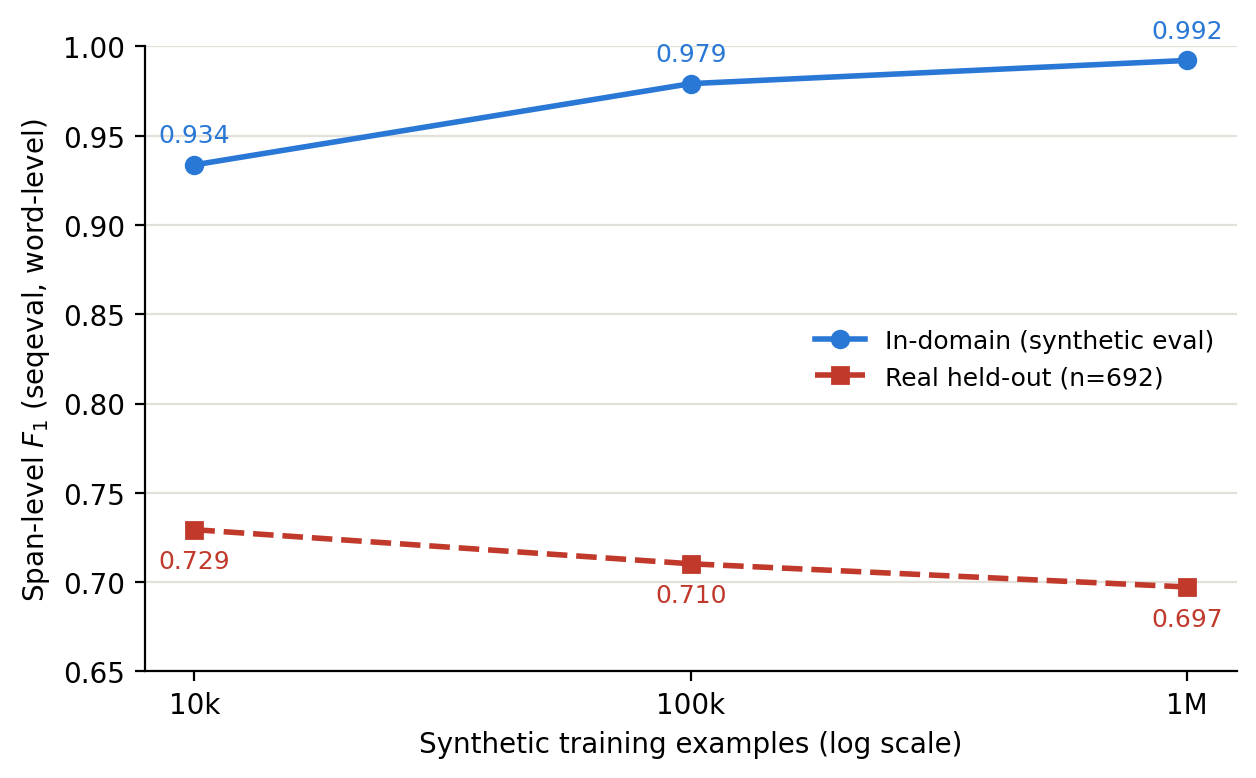
\includegraphics[width=0.8\textwidth]{figures/synthetic_scale_ablation.png}
\caption{Synthetic-scale ablation. In-domain $F_1$ rises with synthetic volume while real held-out $F_1$ falls: more synthetic data fits the corruption distribution more tightly at a small cost to real-data transfer.}
\label{fig:scale_ablation}
\end{figure}

This result should be read with two cautions. First, each row is a single seed, and the real-$F_1$ spread across the whole sweep ($0.032$) is of the same order as the bootstrap confidence intervals in Table~\ref{tab:ling_baseline_ci}; no single pairwise gap is individually significant, and a consistently ordered three-point trend is suggestive but not conclusive (under pure noise, any particular ordering of three points has probability $1/6$). What lends the pattern credibility is that it runs opposite to the in-domain trend, and that it is corroborated by the multi-seed analyses below and by the real-only-from-scratch comparison of Section~\ref{sec:eval_ling_scratch}. Second, the stage-2-versus-final difference of Section~\ref{sec:eval_ling_real} was re-examined in a multi-seed paired analysis (Table~\ref{tab:ling_multiseed}). For each of three additional seeds, the stage-2 checkpoint and the final curriculum model were compared on identical bootstrap resamples of the evaluation set. At the headline synthetic pool, the paired differences on the real split are $+0.016$, $-0.011$, and $+0.003$. The curriculum was then retrained at the ablation-optimal $10^4$ pool for the same three seeds and evaluated both on the real split and on the FCE test set; because the real split was itself used to select that scale, a positive result there would only be suggestive, whereas FCE was never consulted during scale selection and is the independent confirmation set. All nine 95\% intervals straddle zero, and at the $10^4$ scale the mean paired difference is in fact slightly negative ($-0.008$ real, $-0.005$ FCE): even at the synthetic volume most favorable to real-data transfer, and even on the split that chose it, the combined stage~3 yields no reliable paired gain over the stage-2 checkpoint. The single-seed $+4.2$-point difference of Section~\ref{sec:eval_ling_real} is therefore best read as the favorable end of a distribution centered near zero, not as a stable effect. What this comparison cannot show is whether the synthetic stages help relative to training on real data alone, because both checkpoints share the synthetic stage~1. That question, the one H2 poses, is addressed next.

\begin{table}[ht]
\centering
\caption[Multi-seed paired comparison of the stage-2 checkpoint against the full curriculum model.]{Multi-seed paired comparison of the stage-2 checkpoint (synthetic pre-training followed by real fine-tuning) against the full curriculum model (final), word-level span $F_1$ with paired bootstrap 95\% intervals (2{,}000 sentence resamples). Real split $n=692$; FCE test $n=383$. The real split was used to select the $10^4$ scale; FCE was not, making it the independent confirmation set. Every interval straddles zero.}
\label{tab:ling_multiseed}
\begin{tabular}{llccccc}
\toprule
\textbf{Synthetic pool} & \textbf{Eval set} & \textbf{Seed} & \textbf{Stage-2 $F_1$} & \textbf{Final $F_1$} & \textbf{$\Delta$} & \textbf{95\% CI} \\
\midrule
$10^6$ & real & 1 & 0.681 & 0.696 & $+0.016$ & $[-0.009, 0.039]$ \\
$10^6$ & real & 2 & 0.703 & 0.693 & $-0.011$ & $[-0.035, 0.014]$ \\
$10^6$ & real & 3 & 0.663 & 0.666 & $+0.003$ & $[-0.022, 0.029]$ \\
\midrule
$10^4$ & real & 1 & 0.730 & 0.722 & $-0.008$ & $[-0.025, 0.010]$ \\
$10^4$ & real & 2 & 0.728 & 0.714 & $-0.014$ & $[-0.033, 0.004]$ \\
$10^4$ & real & 3 & 0.690 & 0.689 & $-0.001$ & $[-0.020, 0.018]$ \\
\midrule
$10^4$ & FCE  & 1 & 0.687 & 0.679 & $-0.008$ & $[-0.034, 0.018]$ \\
$10^4$ & FCE  & 2 & 0.703 & 0.691 & $-0.012$ & $[-0.036, 0.012]$ \\
$10^4$ & FCE  & 3 & 0.683 & 0.688 & $+0.006$ & $[-0.020, 0.031]$ \\
\bottomrule
\end{tabular}
\end{table}

\subsection{Real-Only Baseline Trained From Scratch}
\label{sec:eval_ling_scratch}

The comparisons above all involve models that were pre-trained on synthetic data: the stage-2 checkpoint is the stage-1 synthetic model fine-tuned on real data (Section~\ref{sec:impl_ling_training}), so stage-2-versus-final measures only the marginal value of the combined stage~3. H2 asks whether synthetic pre-training helps relative to training on the scarce real data alone, and answering that requires a baseline with no synthetic stage. This baseline was trained for four seeds and compared against the curriculum at both the headline $10^6$ pool and the ablation-optimal $10^4$ pool (seeds 1--3, the seeds for which $10^4$ curriculum models exist; Table~\ref{tab:ling_multiseed}): DeBERTa-v3-base initialized from the public pretrained checkpoint and fine-tuned on the real training pool only, under exactly the stage-2 configuration (8 epochs, learning rate $2\times10^{-5}$, 10\% warmup, gradient clipping at 1.0, batch size 16, fp32, focal loss with the same class weights). For each seed, the real 90/10 split is the same one used by the curriculum run with that seed, so the real-only model and each curriculum model are compared on identical evaluation sentences, with the difference computed paired on 2{,}000 sentence-level bootstrap resamples under the word-level span protocol of Table~\ref{tab:ling_baseline_ci}.

\begin{table}[ht]
\centering
\caption[Real-only training from scratch versus the synthetic-to-real curriculum.]{Real-only training from scratch (no synthetic stage) versus the synthetic-to-real curriculum at the headline ($10^6$) and the ablation-optimal ($10^4$) synthetic pools, word-level span $F_1$ on the identical real evaluation split ($n=692$) for each seed, with paired bootstrap 95\% intervals (2{,}000 resamples). $\Delta$ = curriculum $-$ real-only; negative values favor real-only training. No $10^4$ curriculum model exists for seed 0.}
\label{tab:ling_scratch}
\small\setlength{\tabcolsep}{4pt}
\begin{tabular}{ccccccc}
\toprule
\textbf{Synthetic pool} & \textbf{Seed} & \textbf{Real-only $F_1$} & \textbf{Curriculum $F_1$} & \textbf{$\Delta$} & \textbf{95\% CI} & \textbf{$P(\Delta \leq 0)$} \\
\midrule
$10^6$ & 0 & 0.729 & 0.692 & $-0.037$ & $[-0.070, -0.004]$ & 0.983 \\
$10^6$ & 1 & 0.721 & 0.696 & $-0.025$ & $[-0.054, +0.003]$ & 0.958 \\
$10^6$ & 2 & 0.725 & 0.693 & $-0.032$ & $[-0.064, -0.001]$ & 0.978 \\
$10^6$ & 3 & 0.736 & 0.666 & $-0.070$ & $[-0.105, -0.034]$ & 1.000 \\
\midrule
$10^4$ & 1 & 0.721 & 0.722 & $+0.001$ & $[-0.025, +0.025]$ & 0.480 \\
$10^4$ & 2 & 0.725 & 0.714 & $-0.011$ & $[-0.034, +0.011]$ & 0.839 \\
$10^4$ & 3 & 0.736 & 0.689 & $-0.047$ & $[-0.077, -0.016]$ & 1.000 \\
\bottomrule
\end{tabular}
\end{table}

At the headline pool the result (Table~\ref{tab:ling_scratch}) is unambiguous in direction: in every seed, the model trained on the real training split alone (the 6{,}915-sentence pool minus the 692 held-out evaluation sentences) outperforms the full $10^6$ curriculum by 2.5 to 7.0 $F_1$ points, and in three of the four seeds the paired 95\% interval excludes zero. At that volume, synthetic pre-training does not improve real-data detection; it lowers it. This is consistent with the scale ablation (real-data $F_1$ falling as synthetic volume grows) and with the null stage-2-versus-final differences: the synthetic stages move the model toward the corruption distribution, and subsequent real fine-tuning does not fully recover from that.

At the ablation-optimal $10^4$ pool the penalty shrinks but no gain appears: the paired differences are $+0.001$, $-0.011$ and $-0.047$, with two intervals straddling zero and one (seed 3) excluding it on the negative side. The most favorable reading is that a small synthetic pool is, in two of three seeds, statistically indistinguishable from real-only training; in no seed does the curriculum reliably exceed it. Taken together with the $10^6$ rows, the picture is a dose-response one: the more synthetic data precedes real fine-tuning, the further the model ends up below the real-only reference.

Two caveats bound the reading. First, the $10^4$ comparison rests on three seeds, one of which is an outlier in the negative direction; more seeds would tighten the parity claim. Second, the real-only models are evaluated in their training domain; whether synthetic pre-training helps or hurts under domain shift (Holbrook) was not tested from scratch. Within these bounds, H2 is not supported at either evaluated volume (Section~\ref{sec:eval_discuss_hyp}).

\section{Mathematical Error Detection Results}
\label{sec:eval_math}

The mathematical module is evaluated by comparing exact symbolic simulation with the feature-based classifier on three questions. The first is how each method does on clean answers that follow the modeled malrules. The second is how each holds up when those answers are perturbed. The third is how the design of a diagnostic item decides whether different misconceptions can be told apart.

\subsection{Clean Malrule Answers}
\label{sec:eval_math_clean}

On the held-out, stratified 30\% test split of the 1{,}000{,}000 generated problems per operation family, whose incorrect answers follow modeled malrules exactly (ambiguous SFL/BORROW\_NO\_DEC collisions filtered; Section~\ref{sec:impl_math_malrule}), both methods are near-ceiling: the symbolic detector achieves accuracy $1.000$ and the gradient-boosted classifier accuracy $0.997$ (macro-$F_1$ $0.800$ and $0.797$ respectively; the gap between macro-$F_1$ and accuracy is an artifact of including the \texttt{OTHER\_ERROR} class, which never occurs in this test set, in the macro average with a score of zero, not a property of the methods). On answers that exactly follow a known buggy procedure, exact simulation is unbeatable by construction, and the classifier nearly matches it. Both figures characterize correctness under the modeled synthetic conditions, not diagnostic accuracy on real student work, which was not evaluated.

\subsection{Robustness Under Perturbation}
\label{sec:eval_math_noise}

The methods separate sharply under realistic noise. When a $\pm 1$ digit slip is added to each malrule answer, which models a student who applies a buggy procedure and also makes an incidental arithmetic error, the symbolic detector's accuracy collapses to $0.0$ (it requires exact matches by construction), while the ML classifier retains $61.7\%$ accuracy. This is the main precision-versus-robustness trade-off for RQ3: symbolic malrule detection offers exactness and interpretability but has zero tolerance to deviation, while a simple feature-based classifier degrades gracefully. A deployed system should treat them as complements. Exact matches yield high-confidence, interpretable diagnoses, and the classifier is a fallback for answers where no malrule matches exactly.

\subsection{Diagnostic Item Design: Malrule Distinguishability}
\label{sec:eval_math_distinguish}

A third experiment generalizes an incidental finding from dataset generation (Section~\ref{sec:impl_math_malrule}): whether a misconception can be identified from an answer at all depends on the structure of the problem posed. For each problem structure (operand digit count, with and without forcing a borrow-through-zero), 5{,}000 problems were generated and every malrule's simulated answer compared against all others'. Table~\ref{tab:distinguish} reports the fraction of problems on which all three subtraction malrules produce mutually distinct answers (also distinct from the correct one), that is, problems that can in principle diagnose any of the three misconceptions from a single answer.

\begin{table}[h]
\centering
\caption[Malrule distinguishability by problem structure (5{,}000 generated problems per cell).]{Malrule distinguishability by problem structure (5{,}000 generated problems per cell). ``All 3 distinct'' = SFL, BORROW\_ZERO and BORROW\_NO\_DEC yield pairwise different answers, all different from the correct answer.}
\label{tab:distinguish}
\begin{tabular}{ccccc}
\toprule
\textbf{Digits} & \textbf{Zero-borrow forced} & \textbf{All 3 distinct} & \textbf{SFL unique} & \textbf{SFL$=$BND collisions} \\
\midrule
2 & no  & 0.0\%  & 88.5\% & 11.5\% \\
3 & no  & 4.8\%  & 91.7\% & 8.3\% \\
4 & no  & 14.0\% & 93.4\% & 6.6\% \\
6 & no  & 30.7\% & 96.8\% & 3.2\% \\
2 & yes & 0.0\%  & 88.9\% & 11.1\% \\
4 & yes & 43.5\% & 95.5\% & 4.5\% \\
6 & yes & 74.8\% & 98.4\% & 1.6\% \\
\bottomrule
\end{tabular}
\end{table}

The main result is that two-digit problems can never distinguish all three misconceptions (0\% in both conditions; BORROW\_ZERO is never uniquely identifiable at two digits), while six-digit problems with a forced borrow-through-zero distinguish all three on 74.8\% of items. Distinguishability rises monotonically with digit count, and forcing a zero in the borrow chain raises it about three times at four digits ($14.0\% \rightarrow 43.5\%$) and about 2.4 times at six digits ($30.7\% \rightarrow 74.8\%$). The practical implication is a change of question. Besides asking ``how good is the detector?'', a diagnostic system should ask ``which problems make the misconceptions detectable?'' Item difficulty (more digits, zeros in the minuend) is not an obstacle to diagnosis but a prerequisite for it. This gives the system a concrete item-selection policy for deployment, and it connects to the classical observation that bug diagnosis requires adequately discriminating test items \parencite{VanLehn1990}.

\section{Student Profiling Results}
\label{sec:eval_profile}

Four experiments evaluate the profiling module. The first tests, in simulation, how well known archetypes are recovered as separability and data volume change. The second looks for archetype-like structure in real writing by children (Holbrook), and the third for longitudinal stability of behavioral profiles in real data (ASSISTments). The fourth measures the fidelity of the profiles under domain shift, comparing open-world and closed-world settings.

\subsection{Archetype Recovery: Separability $\times$ Data Volume}
\label{sec:eval_profile_ari}

Figure~\ref{fig:ari_sweep} reports the two-factor simulation experiment: Adjusted Rand Index of KMeans archetype recovery as a function of archetype dominance $d$ (how concentrated each profile's error mass is on its characteristic error types) and total observations per student, averaged over three seeds (180 simulated students, six archetypes).

\begin{figure}[ht]
\centering
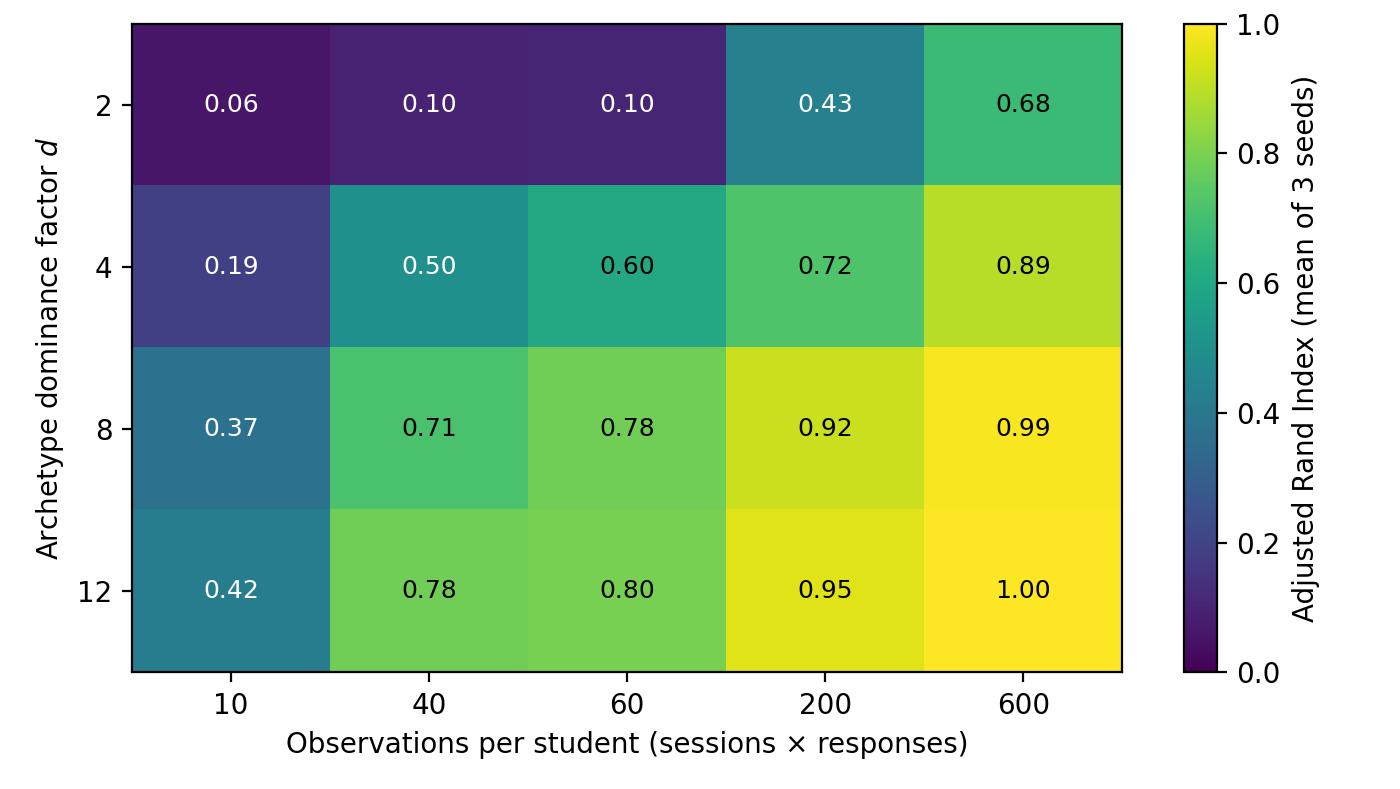
\includegraphics[width=0.85\textwidth]{figures/ari_sweep_heatmap.png}
\caption{Archetype recovery (ARI, mean of 3 seeds) as a function of profile separability ($d$) and observations per student. Recovery requires both factors: neither strong separability with little data nor abundant data on weakly-separated profiles suffices.}
\label{fig:ari_sweep}
\end{figure}

The pattern is monotone in both factors but strongly interactive. With weakly separated profiles ($d=2$), even 600 observations per student reach only ARI $0.68$; with sharply separated profiles ($d \geq 8$), 200 observations suffice for ARI $> 0.9$, and recovery is close to perfect at 600. At realistic classroom volumes (tens of responses per student), only strongly distinct profiles are recoverable at all (ARI $0.37$--$0.78$ at 10--60 observations for $d \geq 8$). For deployment, this means that a system of this kind needs on the order of a few hundred labeled responses per student before its profile clusters can be trusted, unless the underlying difficulty profiles are already sharply distinct.

\subsection{Real Archetype Shapes (Holbrook)}
\label{sec:eval_profile_holbrook}

Clustering the 19 real per-student error distributions from the Holbrook corpus (error-type proportions plus error density) yields an optimal $k=3$ (silhouette $0.338$) with clearly interpretable centroids:

\begin{table}[h]
\centering
\caption{Real per-student clusters in the Holbrook corpus ($k=3$).}
\label{tab:holbrook_clusters}
\begin{tabular}{lrcccc}
\toprule
\textbf{Cluster} & \textbf{n} & \textbf{PHONO} & \textbf{ORTHO} & \textbf{SEG} & \textbf{Err.\ density} \\
\midrule
Mild, segmentation-leaning & 6 & 0.34 & 0.49 & 0.17 & 0.023 \\
Orthographic-dominant, high density & 8 & 0.34 & 0.60 & 0.05 & 0.060 \\
Phonological-dominant, high density & 5 & 0.56 & 0.38 & 0.06 & 0.071 \\
\bottomrule
\end{tabular}
\end{table}

Although $n=19$ permits no strong statistical claims, the qualitative finding matters for H3's plausibility: real struggling writers differ systematically in which error type dominates as well as in how many errors they make. In particular, a phonologically-dominant profile, the signature most associated with phonological-deficit accounts of dyslexia \parencite{ShaywitzShaywitz2005}, emerges from unsupervised clustering of real data without being assumed, under the Metaphone-based operationalization of the PHONO/ORTHO boundary (Section~\ref{sec:impl_ling_taxmap}). The derived centroids were exported in a form directly usable as simulation archetype weights; the ARI sweep of Section~\ref{sec:eval_profile_ari}, however, was run with the hand-specified archetypes, so replacing them with the real-data-derived weights is still a next step.

\subsection{Real Longitudinal Stability (ASSISTments)}
\label{sec:eval_profile_assistments}

For the 1{,}519 ASSISTments students with at least 50 responses, clustering per-student behavioral features finds an optimal $k=2$ (silhouette $0.385$) with a clean pedagogical reading:

\begin{table}[h]
\centering
\caption{Behavioral clusters in ASSISTments 2009--10 ($k=2$, raw-feature centroids).}
\label{tab:assistments_clusters}
\begin{tabular}{lcc}
\toprule
\textbf{Feature} & \textbf{``Coping'' (n=1{,}033)} & \textbf{``Struggling'' (n=486)} \\
\midrule
Accuracy & 0.719 & 0.411 \\
Mean attempts per problem & 1.38 & 2.22 \\
Hint-request rate & 0.104 & 0.355 \\
Median first-response time (s) & 25.0 & 16.2 \\
Repeated-failure rate ($\geq 3$ attempts) & 0.069 & 0.156 \\
\bottomrule
\end{tabular}
\end{table}

The struggling cluster answers faster, not slower. This is consistent with impulsive guessing and hint-fishing, a known behavioral signature in the educational data mining literature \parencite{BakerYacef2009}, and not with slow effortful work. The split-half stability test (Section~\ref{sec:impl_profile_real}) yields ARI $= 0.587$ between clusters computed independently from each student's odd- and even-indexed responses. Profile membership is therefore substantially, though not perfectly, stable across independent halves of a student's real history. Difficulty profiles behave as per-student traits with measurable noise, which is the regime in which the ARI sweep says a few hundred observations are needed for reliable clustering.

\subsection{Profile Fidelity Under Domain Shift: Open vs.\ Closed World}
\label{sec:eval_profile_fidelity}

The final experiment connects the linguistic domain gap (Section~\ref{sec:eval_ling_real}) to its downstream consequence for profiling, and quantifies what the screening mode (Sections~\ref{sec:method_models_screening} and~\ref{sec:impl_prototype_screening}) recovers. For each of the 19 Holbrook students, two error-type distributions over \{PHONO, ORTHO, SEG\} were built from the same 1{,}254 parsed sentences (all of each child's sentences, including the error-free ones; the 531-sentence BIO benchmark is the in-scope-error subset): a \emph{closed-world} profile from the target-known, deterministically mapped labels (what screening would produce), and an \emph{open-world} profile from the neural model's free-text detections.

The two profiles agree grossly in shape (mean cosine similarity $0.882$) but the aggregate hides the failure that matters most pedagogically. Ranking students, which is what a teacher's attention allocation uses, survives for error volume but not for error type: the Spearman rank correlation between open- and closed-world student orderings is $0.898$ for overall error density, but only $0.311$ for the PHONO proportion, $0.179$ for ORTHO, and $0.618$ for SEG. Under domain shift, the open-world detector still identifies almost perfectly which students err a lot, but it largely loses in which way they err, and the error-type mix is what distinguishes difficulty profiles from generic low performance.

This result completes the argument for the two-regime design: passive monitoring remains reliable for volume-based signals and same-domain deployments, while type-resolved profiling of the target population should be grounded in closed-world screening. Screening needs no model inference and so is not subject to training-population shift by construction, though it remains dependent on the mapper's operationalization and on the item bank.

\section{Discussion}
\label{sec:eval_discuss}

The results above are interpreted here in three parts. The hypotheses of Chapter~\ref{chap:introduction} are checked against the evidence, the findings are set against prior work, and the limitations and threats to validity that bound the conclusions are discussed.

\subsection{Hypotheses Revisited}
\label{sec:eval_discuss_hyp}

\textbf{H1} (detection of pedagogically meaningful errors): supported in its testable part, with a quantified domain gap. The mathematical module identifies modeled procedural bugs almost perfectly on clean generated answers, and the linguistic module reaches span-level $F_1 = 0.642$ on real learner text, a demanding metric (exact span and type). However, transfer to the target population is partial ($F_1 = 0.397$ on Holbrook), and the direction of its errors (over-flagging phonological, under-flagging orthographic spans) is itself interpretable in terms of the taxonomy. The part of H1 that refers to consistency with expert teacher annotations was not tested: no teacher-annotation or inter-annotator study was conducted, and performance is measured against the expert-produced gold annotations of the public corpora. ``Pedagogically meaningful'' is therefore supported in the sense that the detected categories are those of an instructionally grounded taxonomy, not in the sense of validated teacher agreement.

\textbf{H2} (synthetic data mitigates scarcity): not supported. Three lines of evidence converge. The direct test, real-only training from scratch versus the curriculum on identical real evaluation sentences with a paired bootstrap, shows the $10^6$ curriculum below real-only training in every one of four seeds, by 2.5 to 7.0 $F_1$ points, with three of four intervals excluding zero; at the $10^4$ pool the curriculum matches real-only training in two of three seeds and falls significantly below it in the third, never exceeding it (Table~\ref{tab:ling_scratch}). The scale ablation shows real-data performance declining as synthetic volume grows ($0.729 \rightarrow 0.697$ over $10^4 \rightarrow 10^6$), the opposite of the in-domain trend (Table~\ref{tab:ling_scale}). And the nine paired stage-2-versus-final comparisons are centered near zero (Table~\ref{tab:ling_multiseed}), so the combined stage does not compensate. The reading supported by the evidence is that rule-based synthetic data of the kind generated here does not improve on real data under the evaluated conditions (at best it is neutral at small volumes), and that its effect on real-data transfer worsens with volume; more synthetic examples fit the corruption distribution, not the target one. This is a negative result, but a design-relevant one: under a fixed real budget, the limiting factor is the match between synthetic and target error distributions, not data amount, and generating more of a mismatched distribution is counterproductive.

\textbf{H3} (interpretable difficulty profiles): partially supported, with structural evidence from three complementary sources and pedagogical meaningfulness untested. The evidence covers recoverability (simulation, with quantified data requirements), the existence of archetype-like structure in real struggling writers (Holbrook, $n=19$, silhouette $0.338$), and longitudinal stability (ASSISTments split-half ARI 0.587). Two qualifications apply. The ASSISTments profiles are built from behavioral features (accuracy, attempts, hints, response time), not from error-type detections of this system, so they establish that per-student profiles of the kind the module computes can be stable traits, not that this system's error-type profiles are. And the ``meaningful and actionable for educators'' component of H3 was not tested with any educator; interpretability was assessed by centroid inspection only. None of the three sources alone would suffice; together they support the structural claims a simulation-only validation could not, while leaving the pedagogical claim to the pilot proposed in Chapter~\ref{chap:Chapter6}.

\subsection{Relation to Prior Work}
\label{sec:eval_discuss_prior}

Cross-corpus evaluation of error-correction systems is an established concern: \textcite{Mita2019CrossCorpora} showed that single-corpus GEC evaluation overstates robustness across L2 learner corpora, and \textcite{Flachs2020CWEB} extended the argument to low-error-density native web text. This thesis's domain-shift evaluation differs on two axes. First, the shift is toward writers with literacy difficulties, the population that educational error detection serves and that the dyslexia literature has studied mainly through handwriting-image classification or resource building \parencite{RelloBaezaYates2014}, not through text-based detector transfer. Second, the analysis is resolved to the level the application needs: it decomposes the downstream per-student profiles into volume fidelity (preserved: Spearman $0.898$) and type fidelity (lost: $0.18$--$0.62$) instead of reporting one aggregate score. To the best of our knowledge, this volume-versus-type characterization of domain shift in educational error detection has not been reported before, and it directly changes the system design conclusion (two-regime routing) rather than merely qualifying a benchmark number.

\subsection{Limitations}
\label{sec:eval_discuss_limit}

\begin{itemize}
    \item The training data do not match the target population: both real GEC corpora contain adult L2 writing, and the 20-point Holbrook drop measures the cost. No public error-annotated corpus of children with learning difficulties exists at training scale, and collecting one (with ethics approval) is the highest-value future step.
    \item The target-population benchmark is small. Holbrook has 19 writers and 531 usable sentences from a 1964 British classroom; conclusions drawn from it are directional, not definitive.
    \item All experiments are English-language; the architecture is language-agnostic but the resources (corpora, homophone lexicon, Metaphone) are not.
    \item The scope is non-clinical. The system detects error patterns and behavioral profiles, not learning disabilities; no clinical validation is claimed or attempted. Profiles are formative-assessment aids for teachers.
    \item Type-resolved profiles from free text inherit the domain gap. The fidelity experiment shows open-world detections preserve volume rankings (Spearman $0.898$) but not type rankings ($0.18$--$0.62$) on the target population; profiles built from free writing alone should therefore be treated as volume-reliable and type-tentative until the gap is closed or screening data is available.
    \item Outside the simulation, no gold difficulty-profile labels exist; the real-data studies validate structure (archetypes exist, profiles are stable) rather than accuracy against known truth.
    \item The mathematical evaluation uses generated data only. All mathematical results (clean accuracy, robustness under a modeled digit slip, distinguishability) are computed on generated malrule answers; no real student arithmetic responses were evaluated. The figures characterize correctness and discrimination under the modeled conditions, not diagnostic accuracy in classrooms.
    \item Neither the detections nor the profiles were reviewed by teachers, and no inter-annotator study was run; the ``pedagogically meaningful'' and ``actionable'' components of H1 and H3 rest on the taxonomy's grounding, not on measured teacher agreement.
\end{itemize}

\subsection{Threats to Validity}
\label{sec:eval_discuss_threats}

For internal validity, the learning rate, warmup and gradient clipping were fixed to make training numerically stable rather than by searching for $F_1$ (Section~\ref{sec:impl_ling_training}), and epoch counts were scaled with dataset size. One selection did use evaluation data: the $10^4$ synthetic scale was chosen on the real evaluation split, which can make that pool's real-split figure optimistic, so the FCE test split, not used for selection, is the independent check. The taxonomy mapper is deterministic, but its category boundaries (e.g., Metaphone equality for PHONO/ORTHO) are one operationalization among several defensible ones, and per-category results depend on it. For external validity, results may not generalize across languages, age groups, or educational contexts, and the ASSISTments students used one particular tutoring system whose hint economy shapes behavior. For construct validity, ``difficulty profiles'' are proxies built from observable errors, not measurements of underlying cognitive constructs, and the Holbrook error annotations reflect one annotator's (the original teacher's) transcription fidelity.

\section{Summary}
\label{sec:eval_summary}

The evaluation established that: (i) synthetic pre-training at the evaluated volume ($10^6$) does not improve on real-only training (in four paired seeds the curriculum is 2.5--7.0 $F_1$ points below a model trained from scratch on the real pool alone, the combined stage adds nothing reliable, and real-data performance falls as synthetic volume grows while in-domain performance rises), and at the $10^4$ pool the curriculum at best matches real-only training (two of three seeds) and never exceeds it, so H2 is not supported; (ii) on generated malrule data, exact symbolic detection and a simple ML classifier are complementary, with a stark precision-robustness trade-off (100\% vs.\ 0\% on clean/perturbed for the symbolic method, against 99.7\%/61.7\% for the classifier), and misconception identifiability depends on problem structure; (iii) difficulty-profile clustering is supported structurally from three angles (recoverable in simulation with quantified data requirements, present as archetype-like shapes among 19 real struggling writers, and stable across independent halves of real longitudinal behavioral histories), though without educator validation; and (iv) the dominant open problem is the domain gap to the target population, quantified here at roughly 20 $F_1$ points, under which free-text detection preserves error-volume rankings but not error-type rankings. The final chapter draws conclusions and outlines future work.

% Chapter 6

\chapter{Conclusions and Future Work} % Main chapter title
\label{chap:Chapter6} % For referencing the chapter elsewhere, use \ref{chap:Chapter6}

%----------------------------------------------------------------------------------------

This chapter summarizes the research contributions (Section~\ref{sec:concl_contrib}), revisits the research questions and hypotheses against the experimental evidence (Section~\ref{sec:concl_rq}), consolidates the limitations (Section~\ref{sec:concl_limit}), and outlines future work (Section~\ref{sec:concl_future}). The domain gap to the target population, quantified in Chapter~\ref{chap:Chapter5}, is treated throughout as the main open problem.

\section{Summary of Contributions}
\label{sec:concl_contrib}

This thesis addressed the automatic detection of error patterns linked to learning difficulties in typed student responses. Its contributions are of three kinds: empirical results, reusable methodological findings, and a working system.

The first contribution is an operational taxonomy with an audited mapping from public corpora. The three-category linguistic taxonomy (phonological, orthographic, segmentation) was made operational through a deterministic mapper from ERRANT-annotated GEC corpora. The mapper was audited against $\sim$65{,}000 real gold edits, and the audit caught three plausible-looking but wrong mapping rules. Beyond the taxonomy itself, the practical contribution is the demonstrated route from generic public GEC annotations to difficulty-oriented labels.

The synthetic-data hypothesis received a quantified, negative answer. The direct test compared real-only training from scratch with the full synthetic-to-real curriculum on identical real evaluation sentences (four seeds, paired bootstrap). At the headline $10^6$ synthetic pool the curriculum lands 2.5--7.0 $F_1$ points below real-only training, with three of four intervals excluding zero. The scale ablation shows real-data transfer degrading as synthetic volume grows while in-domain performance rises, and nine paired stage-2-versus-final comparisons show that the combined stage adds nothing reliable. At the ablation-optimal $10^4$ pool the same paired comparison finds no gain either: parity in two of three seeds, and in the third a loss whose interval excludes zero. Under the evaluated conditions, then, rule-based synthetic data of the kind generated here does not improve on scarce real data. At best it is neutral at small volumes, and generating more of it is counterproductive. The match between synthetic and authentic error distributions, not volume, is the limiting factor.

For mathematical misconceptions, the thesis measures a trade-off between symbolic and ML methods and reports an item-design result. On generated answers that follow the modeled malrules exactly, symbolic simulation is perfect and a gradient-boosted classifier nearly matches it (accuracy 0.997). Under a one-digit slip superimposed on the malrule answer, the symbolic method collapses to 0\% by construction while the classifier retains 61.7\%. The item-design result concerns malrule \emph{distinguishability}, which depends on problem structure: two-digit subtraction can never separate the three modeled bugs, while six-digit problems with a forced borrow-through-zero separate all three in 74.8\% of items. Item structure is therefore a diagnostic design variable.

Difficulty profiling under data absence rests on a three-way evidence design. No public dataset offers longitudinal, difficulty-labeled, per-student responses, so profiling was assessed from three directions: recoverability of known archetypes in simulation (with a two-factor experiment quantifying how many observations per student reliable clustering requires); the existence of archetype-like shapes among 19 real struggling child writers (including an unsupervised-emergent phonologically-dominant profile consistent with phonological-deficit accounts of dyslexia, under the thesis's operationalization of the phonological/orthographic boundary); and the split-half stability of behavioral profiles on 1{,}519 real students (ARI 0.587). This design supports the structural claims of H3. It does not validate the profiles against educator judgment or any external construct.

The engineering lessons are documented as well. The implementation chapters record the full decision path, including failed intermediate attempts: the loss-function progression forced by extreme class imbalance (plain and weighted cross-entropy each collapsing in opposite directions before focal loss stabilized training), silent numerical failure modes (fp16 checkpoint loading without loss scaling), and two evaluation-design failures (template memorization; synthetic-dominated evaluation sets) that produced misleadingly high scores before being diagnosed. Similar educational-NLP efforts can reuse these as warnings.

The two-regime detection design comes with a measured justification. Worksheet items have known targets, so the system routes closed-world responses to a deterministic, domain-gap-free scorer over diagnostically selected items (screening) and reserves the neural model for open-world free text (monitoring). The profile-fidelity experiment justifies the split empirically. Under domain shift, free-text detection preserves student rankings by error volume (Spearman $0.898$) but not by error type ($0.18$--$0.62$), and screening recovers the type-resolved signal that free text loses.

The last contribution is a pilot-ready prototype with a bilingual screening mode and an explicit ethical framing. The thin web prototype (student exercise flow; teacher dashboard over the profiling representation) demonstrates the full pipeline end-to-end and surfaced two deployment findings that the benchmarks had not (confidence thresholding; tokenization-contract violations). It also embodies the thesis's non-clinical posture: local-only storage, formative vocabulary, teacher interpretation required. The screening mode runs in both English and European Portuguese. The Portuguese instantiation (item bank plus purpose-built phonetic comparator, validated by unit and archetypal tests and a reproducible case-study walkthrough) delivers the portability claim the two-regime design makes, in the thesis's original motivating language.

\section{Revisiting Research Questions and Hypotheses}
\label{sec:concl_rq}

The research questions come first, followed by the hypotheses, and both are judged against the experimental evidence of Chapter~\ref{chap:Chapter5}. Each hypothesis verdict states whether the evidence supports the claim and where that evidence is still incomplete.

\subsection{Research Questions}
\label{sec:concl_rq_questions}

\textbf{Q1} (linguistic error taxonomies). The three-category taxonomy proved operationalizable at scale, and its categories also exist in real struggling writers' data. Clustering the Holbrook children's per-student error distributions yields groups distinguished by dominant category (phonological-dominant, orthographic-dominant, mild/segmentation-leaning), a structure that no analysis step assumed in advance. Prevalence differs by population. Orthographic errors are over-represented among struggling child writers relative to adult L2 learners, and this is what the domain-shift experiment exposed.

\textbf{Q2} (detection and classification models). Supported with quantified boundaries. The final model reaches span-level $F_1 = 0.642$ on real learner text under a strict exact-span, exact-type metric, and $0.594$ on a fully held-out same-domain benchmark. On the target population (Holbrook), performance drops to $0.397$; automated detection is practical within the training domain and measurably degraded outside it. Comparison against human inter-annotator agreement remains future work, as no such annotation study was run.

\textbf{Q3} (mathematical misconception detection). The answer is a trade-off with two sides. Symbolic methods are exact and interpretable on modeled bugs but brittle to any deviation, while a simple ML classifier is marginally less exact and far more robust (61.7\% vs.\ 0\% under answer noise). The two methods complement each other. The distinguishability experiment adds that what the system can diagnose is bounded by which problems it poses.

\textbf{Q4} (data scarcity and synthesis). Under the evaluated conditions, the synthetic curriculum was not the most effective training set. Fine-tuning on the real training split alone outperformed the full curriculum at $10^6$ synthetic examples in every seed. Among curriculum variants, a modest synthetic pool ($10^4$ examples) transferred best, and scaling to the million-sentence level improved only in-domain performance while degrading real-data transfer. Tested directly against real-only training, that small pool was neutral in two of three seeds and worse in the third, never better. LLM-based augmentation was considered and not adopted (label reliability, cost at scale, sufficiency of rules for the surface-realizable taxonomy). The current generator falls short on fidelity to authentic error distributions, both for the adult learner corpora (as the from-scratch comparison shows) and for the target population (as the domain gap shows).

\textbf{Q5} (difficulty profiling). Aggregated error patterns do cluster into stable, interpretable profiles. This comes with quantified preconditions, and their pedagogical meaningfulness to educators has not yet been assessed. Simulation shows that reliable recovery (ARI $> 0.9$) requires either sharply distinct profiles or a few hundred observations per student. Real behavioral data shows two cleanly interpretable clusters (``coping'' vs.\ ``struggling'', the latter marked by faster, hint-heavy, repeated-failure responding) with substantial but imperfect split-half stability (ARI 0.587). The prototype's dashboard presents profiles in the intended non-clinical format. Its screening mode addresses the practical question behind Q5, which is how quickly a teacher can get a signal: one or two worksheets are meant to yield a type-resolved \emph{screening} flag (closed-world scoring of diagnostically selected items; not yet validated with children), while stable \emph{profiles} still require the longitudinal accumulation the ARI experiment quantifies.

\subsection{Hypotheses}
\label{sec:concl_rq_hyp}

\textbf{H1} is supported in its testable part, with a quantified domain boundary. NLP and symbolic methods identify the error types of the instructionally grounded taxonomy under strict metrics, and the mathematical module identifies modeled procedural bugs with near-perfect accuracy on clean generated answers. The claim ``performance consistent with expert teacher annotations'' could not be tested directly (no annotation study). What was tested and quantified is performance against gold corpus annotations, including on the target population, where the 20-point drop marks the current boundary of validity.

\textbf{H2} is not supported. Against real-only training from scratch on identical real evaluation data, the $10^6$ curriculum is 2.5--7.0 $F_1$ points worse in each of four seeds (three of four paired intervals excluding zero). The $10^4$ curriculum is at best neutral (parity in two of three seeds, significantly worse in the third). The scale ablation shows real-data performance declining as synthetic volume grows, and nine paired stage-2-versus-final comparisons show the combined stage adds nothing reliable. The claim the evidence supports is the negative, design-relevant one from Chapter~\ref{chap:Chapter5}: under a fixed real-data budget, rule-based synthetic data of the kind generated here does not substitute for real data, and past a modest volume the limiting factor is error type-match, not data amount. The hypothesis as originally stated included LLM-based generation, which was not adopted, so the evidence addresses the rule-based half of the hypothesis and leaves the LLM half untested.

\textbf{H3} is partially supported. The structural evidence converges, but pedagogical validation is pending. No single dataset could test H3; the combination of simulation recoverability, archetype-like structure in real struggling writers, and longitudinal stability of behavioral profiles covers its structural claims. Two components remain untested. One is the ``meaningful and actionable for educators'' component, which no educator has assessed. The other is the full loop on the target population, meaning profiles built from this system's own detections on real children's responses over a school term. Both require the pilot deployment outlined below.

\section{Limitations}
\label{sec:concl_limit}

The limitations documented throughout Chapters~3--5 come down to six:

\begin{itemize}
    \item The domain gap to the target population is the dominant limitation. All real training data is adult L2 learner writing; on real struggling child writers, detection $F_1$ drops from $\sim$0.6 to $\sim$0.4, with a diagnostic error signature (phonological over-prediction, orthographic under-prediction). Every claim in this thesis about the target population inherits this boundary.
    \item The benchmark for that population is limited in size and provenance. The only located target-population benchmark (Holbrook) comprises 19 writers and 531 sentences from a 1964 British classroom, transcribed by their teacher. It is directionally informative but statistically thin.
    \item Free-text experiments cover English only. The trained model, the corpora, and the homophone lexicon are English resources, and Portuguese free-text deployment, the original motivating context, still requires Portuguese data end to end. The screening regime is the exception: its European Portuguese instantiation (item bank plus phonetic comparator, Section~\ref{sec:impl_prototype_screening_pt}) runs end to end and passes its archetypal test suite, though it has not yet been administered to children.
    \item The scope is non-clinical, by design. Profiles are statistical constructs over observable errors. No clinical validation was attempted, none is claimed, and the system's outputs are framed accordingly. This is an ethical stance, and it also matches what the evidence supports.
    \item The mathematical results use generated data only. Every mathematical figure (clean accuracy, robustness to a modeled digit slip, distinguishability) is computed on generated malrule answers, and no real student arithmetic was evaluated. The results characterize the methods under the modeled conditions, not classroom diagnostic accuracy.
    \item No educator has validated the work. Detections, taxonomy categories, and profiles were not reviewed by teachers, and no inter-annotator study was conducted. The ``pedagogically meaningful'' and ``actionable'' components of H1 and H3 rest on the taxonomy's grounding in the literature, not on measured teacher agreement; the pilot below is where that evidence would come from.
\end{itemize}

\section{Future Work}
\label{sec:concl_future}

Future work follows from the limitations above. The domain gap to the target population comes first because it is the main open problem. After it come the validation of the screening instrument, a school pilot, support for Portuguese, and a set of broader extensions of the approach.

\subsection{Closing the Domain Gap}
\label{sec:concl_future_gap}

The 20-point Holbrook drop defines the highest-value research direction, approachable on three fronts in increasing order of cost:
\begin{enumerate}
    \item The generator can be matched to the target population. It currently corrupts text uniformly, and the from-scratch comparison shows that more of that distribution hurts. The Holbrook analysis provides real per-population error distributions (category proportions, density) that the generator could target instead, and the natural next test is whether better-matched synthetic data can help even without more of it. LLM-based generation, rejected for the uniform case, becomes attractive here: generating text with a specified population's error signature is what conditional generation is for.
    \item Even tens of in-domain sentences (an ethics-cleared micro-pilot) could support few-shot adaptation, through continued fine-tuning or adapter layers, evaluated against the Holbrook benchmark already in place.
    \item The definitive fix is an in-domain corpus: an ethics-approved collection of typed responses from the target population, difficulty-annotated with teacher input. It is costly, but the thesis's pipeline (taxonomy mapper, BIO conversion, benchmarks) makes every collected sentence immediately usable.
\end{enumerate}

\subsection{Validating the Screening Instrument}
\label{sec:concl_future_screening}

The screening item bank rests on principled but unvalidated item selection. The discriminative signature of each word family is argued from the taxonomy and the mapper's mechanics, and it has not yet been measured on children. A validation study would administer the worksheet to a real class and compare the outcome with teacher judgment. Such a study is small and ethically simple (a normal dictation exercise), and it would also yield the first in-domain data for the adaptation path above. The European Portuguese instantiation of the screening mode (Section~\ref{sec:impl_prototype_screening_pt}) would be validated by the same protocol.

\subsection{School Pilot}
\label{sec:concl_future_pilot}

The prototype makes a concrete pilot protocol possible. It would be deployed locally in one school, with consent and pseudonymization, and would collect (i) real detection precision as experienced by teachers, (ii) the per-student observation counts the ARI experiment identifies as necessary, and (iii) teacher judgments of profile interpretability. The last is the educator-validation step deliberately not claimed in this thesis. The pilot also feeds direction 3 above.

\subsection{Portuguese Support}
\label{sec:concl_future_pt}

The screening half of Portuguese support was delivered within this thesis. Section~\ref{sec:impl_prototype_screening_pt} describes the European Portuguese item bank and grapheme-to-phoneme comparator, and the case-study walkthrough exercises them end to end. It confirms the prediction that the closed-world regime ports with two artifacts and no data. What remains is (i) validating that instantiation with real Portuguese children (the item families and trap words are principled but not yet field-tested), and (ii) the free-text path, which is the expensive half. That path needs a Portuguese encoder (e.g., BERTimbau or multilingual DeBERTa), Portuguese base sentences for the synthetic generator, a Portuguese homophone lexicon, and above all Portuguese error-annotated data. The COPLE2 population mismatch that redirected this thesis remains unsolved and would need addressing, most plausibly via the pilot route.

\subsection{Broader Extensions}
\label{sec:concl_future_broader}

In order of readiness, the first extension is introductory algebra misconceptions, using the expert-validated MaE dataset. The detection architecture transfers, but the item-design analysis would need redoing for each misconception class. Next, detected profiles could be coupled to intervention suggestions, which moves the system from detection toward tutoring \parencite{VanLehn2006}. Handwriting input via OCR/HTR would fit real classroom workflows. The last extension is a set of longitudinal studies, run with educational psychologists, that correlate early detected patterns with later outcomes. That is the eventual bridge between statistical profiles and clinically meaningful categories, and it should never be shortcut.

\section{Concluding Remarks}
\label{sec:concl_final}

This thesis set out to detect error patterns linked to learning difficulties in typed student responses, under the constraint that the data such a system most needs largely does not exist publicly. The results are two-sided.

Symbolic and learned methods for mathematical bugs trade exactness against robustness, which makes them complements, and what they can diagnose depends on the items posed. Difficulty profiles are recoverable in simulation, present as archetype-like structure in real struggling writers, and stable in real longitudinal behavioral data. Under domain shift, free-text detection preserves error-volume rankings while losing error-type rankings, which gives the two-regime design an empirical basis. The whole pipeline runs end to end in a pilot-ready prototype.

There are also two negative results. Rule-based synthetic data did not improve on real-only training at the volume evaluated, and its value is bounded by the match between synthetic and authentic error distributions. A 20-point performance drop on real struggling child writers quantifies how far training on available proxy populations carries, and how far it does not.

The thesis demonstrates the method (a taxonomy, a controlled evaluation of synthetic data, complementary detectors, and multi-source profiling evidence, all reproducible) and measures the distance that remains to the application. It does not claim readiness for classroom use. That measured distance is what makes the next steps (population-targeted generation, a consented school pilot, Portuguese resources) concrete.



%----------------------------------------------------------------------------------------
%	BIBLIOGRAPHY
%----------------------------------------------------------------------------------------

\printbibliography[heading=bibintoc]


%----------------------------------------------------------------------------------------
%	THESIS CONTENT - APPENDICES
%----------------------------------------------------------------------------------------

\appendix % Cue to tell LaTeX that the following "chapters" are Appendices

% Include the appendices of the thesis as separate files from the Appendices folder
% Uncomment the lines as you write the Appendices

% % Appendix A

\chapter{Appendix Title Here} % Main appendix title

\label{AppendixA} % For referencing this appendix elsewhere, use \ref{AppendixA}

This appendix serves as a placeholder for supplementary content.
%\input{appendices/appendixB}
%\input{appendices/appendixC}

%----------------------------------------------------------------------------------------

\end{document}
